\RequirePackage[l2tabu,orthodox]{nag}

% TODO: decide if one-sided/two-sided
%\documentclass[headsepline,footsepline,footinclude=false,fontsize=11pt,paper=a4,listof=totoc,bibliography=totoc,BCOR=12mm,DIV=12]{scrbook} % two-sided
\documentclass[headsepline,footsepline,footinclude=false,oneside,fontsize=11pt,paper=a4,listof=totoc,bibliography=totoc]{scrbook} % one-sided

% TODO: change citation style in settings
\PassOptionsToPackage{table,svgnames,dvipsnames}{xcolor}

\usepackage[utf8]{inputenc}
\usepackage[T1]{fontenc}
\usepackage[sc]{mathpazo}
\usepackage[ngerman,american]{babel}
\usepackage[autostyle]{csquotes}
\usepackage[
  backend=biber,
  url=false,
  style=authoryear,
  sorting=ynt ]{biblatex}
\usepackage{graphicx}
\usepackage{scrhack} % necessary for listings package
\usepackage{listings}
\usepackage{lstautogobble}
\usepackage{tikz}
\usepackage{pgfplots}
\usepackage{pgfplotstable}
\usepackage{booktabs}
\usepackage[final]{microtype}
\usepackage{caption}
\usepackage{subfig}
\usepackage{wrapfig}
\usepackage[hidelinks]{hyperref} % hidelinks removes colored boxes around references and links
\usepackage[acronym, toc]{glossaries}
\makeglossaries
\bibliography{bibliography}
\renewcommand*{\nameyeardelim}{\addcomma\space}
\setkomafont{disposition}{\normalfont\bfseries} % use serif font for headings
\linespread{1.05} % adjust line spread for mathpazo font

\DeclareCiteCommand{\citeauthor}
  {\boolfalse{citetracker}%
   \boolfalse{pagetracker}%
   \usebibmacro{prenote}}
  {\ifciteindex
     {\indexnames{labelname}}
     {}%
   \printtext[bibhyperref]{\printnames{labelname}}}
  {\multicitedelim}
  {\usebibmacro{postnote}}

% Add table of contents to PDF bookmarks
\BeforeTOCHead[toc]{{\cleardoublepage\pdfbookmark[0]{\contentsname}{toc}}}

% Define TUM corporate design colors
% Taken from http://portal.mytum.de/corporatedesign/index_print/vorlagen/index_farben
\definecolor{TUMBlue}{HTML}{0065BD}
\definecolor{TUMSecondaryBlue}{HTML}{005293}
\definecolor{TUMSecondaryBlue2}{HTML}{003359}
\definecolor{TUMBlack}{HTML}{000000}
\definecolor{TUMWhite}{HTML}{FFFFFF}
\definecolor{TUMDarkGray}{HTML}{333333}
\definecolor{TUMGray}{HTML}{808080}
\definecolor{TUMLightGray}{HTML}{CCCCC6}
\definecolor{TUMAccentGray}{HTML}{DAD7CB}
\definecolor{TUMAccentOrange}{HTML}{E37222}
\definecolor{TUMAccentGreen}{HTML}{A2AD00}
\definecolor{TUMAccentLightBlue}{HTML}{98C6EA}
\definecolor{TUMAccentBlue}{HTML}{64A0C8}

% Settings for pgfplots
\pgfplotsset{compat=newest}
\pgfplotsset{
  % For available color names, see http://www.latextemplates.com/svgnames-colors
  cycle list={TUMBlue\\TUMAccentOrange\\TUMAccentGreen\\TUMSecondaryBlue2\\TUMDarkGray\\},
}

% Settings for lstlistings
\lstset{%
  basicstyle=\ttfamily,
  columns=fullflexible,
  autogobble,
  keywordstyle=\bfseries\color{TUMBlue},
  stringstyle=\color{TUMAccentGreen},
  escapeinside={(*@}{@*)}
}

% TODO: change thesis information
\newcommand*{\getUniversity}{Technische Universität München}
\newcommand*{\getFaculty}{Department of Informatics}
\newcommand*{\getTitle}{Optimizing Transmission of 3D Video Data for Limited Bandwidth and Latency through Foveated Rendering and Superresolution}
\newcommand*{\getTitleGer}{Übertragungsoptimierung von 3D Video Material innerhalb eines Bandbreiten und Latenz limitierten Netzwerkes mit Hilfe von Foveated Rendering und Super-Resolution}
\newcommand*{\getAuthor}{Philip Hagemann}
\newcommand*{\getDoctype}{Master's Thesis in Robotics, Cognition, Intelligence}
\newcommand*{\getSupervisor}{Prof. Dr.-Ing. Alois Knoll}
\newcommand*{\getAdvisor}{Rafael Hostettler, Alona Kharchenko}
\newcommand*{\getSubmissionDate}{15. November 2020}
\newcommand*{\getSubmissionLocation}{Munich}

\begin{document}

\pagenumbering{alph}
\begin{titlepage}
  % HACK for two-sided documents: ignore binding correction for cover page.
  % Adapted from Markus Kohm's KOMA-Script titlepage=firstiscover handling.
  % See http://mirrors.ctan.org/macros/latex/contrib/koma-script/scrkernel-title.dtx,
  % \maketitle macro.
  \oddsidemargin=\evensidemargin\relax
  \textwidth=\dimexpr\paperwidth-2\evensidemargin-2in\relax
  \hsize=\textwidth\relax

  \centering

  \IfFileExists{logos/tum.pdf}{%
    
\includegraphics[height=20mm]{logos/tum.pdf}
  }{%
    \vspace*{20mm}
  }

  \vspace{5mm}
  {\huge\MakeUppercase{\getFaculty{}}}\\

  \vspace{5mm}
  {\large\MakeUppercase{\getUniversity{}}}\\

  \vspace{20mm}
  {\Large \getDoctype{}}

  \vspace{15mm}
  {\huge\bfseries \getTitle{}}

  \vspace{15mm}
  {\LARGE \getAuthor{}}

  \IfFileExists{logos/faculty.pdf}{%
    \vfill{}
    \includegraphics[height=20mm]{logos/faculty.pdf}
  }{}
\end{titlepage}

\frontmatter{}

\begin{titlepage}
  \centering

  \IfFileExists{logos/tum.pdf}{%
    
\includegraphics[height=20mm]{logos/tum.pdf}
  }{%
    \vspace*{20mm}
  }

  \vspace{5mm}
  {\huge\MakeUppercase{\getFaculty{}}}\\

  \vspace{5mm}
  {\large\MakeUppercase{\getUniversity{}}}\\

  \vspace{10mm}
  {\Large \getDoctype{}}

  \vspace{10mm}
  {\huge\bfseries \getTitle{} \par}

  \vspace{10mm}
  {\huge\bfseries \foreignlanguage{ngerman}{\getTitleGer{}} \par}

  \vspace{10mm}
  \begin{tabular}{l l}
    Author:          & \getAuthor{} \\
    Supervisor:      & \getSupervisor{} \\
    Advisor:         & \getAdvisor{} \\
    Submission Date: & \getSubmissionDate{} \\
  \end{tabular}

  \IfFileExists{logos/faculty.pdf}{%
    \vfill{}
    \includegraphics[height=20mm]{logos/faculty.pdf}
  }{}
\end{titlepage}

\thispagestyle{empty}
\vspace*{0.8\textheight}
\noindent
I confirm that this \MakeLowercase{\getDoctype{}} is my own work and I have documented all sources and material used.

\vspace{15mm}
\noindent
\getSubmissionLocation{}, \getSubmissionDate{} \hspace{50mm} \getAuthor{}

\cleardoublepage{}

\addcontentsline{toc}{chapter}{Acknowledgments}
\thispagestyle{empty}

\vspace*{20mm}

\begin{center}
{\usekomafont{section} Acknowledgments}
\end{center}

\vspace{10mm}
I would first like to thank my parents and my grandmother for offering wise counsel, a sympathetic ear and endless support.
\par
I would also like to thank my tutors, Rafael Hostettler and Alona Kharchenko, for their valuable guidance throughout my studies. In addition, I would also like to thank the staff behind Roboy  for being part of this incredible project and for allowing me the possibility to write my thesis about this exciting topic.

\cleardoublepage{}

\chapter{\abstractname}
Real-time streaming for telepresence is with current streaming challenging. Real-time streaming becomes essential as with the recent developments in virtual reality, enchanting applications for telepresence are becoming possible. For controlling robots or other time-sensitive tasks, virtual reality represents the robot's view of the natural environment to the user in 3D. However, the robot may be all around the world. One of the main problems is that the user suffers side-effects and cannot control the robot appropriately when the camera stream delays from the robot to the head-mounted display. In this context, telepresence is defined as the status of feeling to be in a distant environment. The higher the immersion of the virtual reality is, the more the user feels to be in that other location. 
\par
This project aims to develop a low latency streaming application that adjusts the stream dynamically to the available bandwidth to provide the best possible image to the user. The difference as compared to streaming used by Netflix or television is that the low latency requirement while having only low bandwidth available in real-time is in a tremendous contrast as low latency requires less computation resulting in a higher transfer rate. However, with the upcoming availability, for example by the HTC VIVE Pro Eye, which predicts the current user's gaze in virtual reality, the transfer rate is reduced to a minimum by a technique named foveated rendering. The solution includes multiple steps: downscaling the video by calculating a foveated rendering, transmitting the video, performing superresolution of the frames of the streamed video, and delivering it to a head-mounted display showing the virtual reality. In this presented application, calculating the foveated rendering is achieved by splitting the foveated area and the peripheral region into two streams with high-resolution and low-resolution. Machine learning performs superresolution of the received background at the client-side to increase the background details. Afterwards, the foveated and the peripheral area are merged and shown to the user. 
\par
The results showed an implementation, which reduces the latency with foveated rendering being considerably lower in comparison to traditional streaming solutions. Furthermore, the quality in the current user's gaze is high when the available bandwidth is low. These results suggest that for performing time-sensitive tasks requiring telepresence, the concept of streaming including foveated rendering and superresolution should be taken into account.
\microtypesetup{protrusion=false}
\tableofcontents{}
\microtypesetup{protrusion=true}


\mainmatter{}

\chapter{Introduction}\label{chapter:introduction}
The capabilities and features of \gls{vr} are continually increasing, and is now capable of providing an immersive feeling. Additionally, developers and users’ interest in telepresence is growing, because it offers many possibilities for people not to be on-site. Telepresence describes the 'the perception of presence within a physically remote or simulated site' \parencite {Draper1998}. For example, as COVID-19 spreads worldwide and people have to stay at home, the need for a social life is still essential for humans but cannot be fulfilled \parencite {Berg2020}. Therefore, the need for social interaction without being in the same location as others is increasing. Another example is climate change. Travelling worldwide for tourism is becoming less popular as flying and driving emit significant levels of CO2 \parencite {Zhang2019}. Solutions such as Skype, Zoom and other video conference applications help mitigate this need, but they are not equal to personal contact \parencite {Judge2010}. Telepresence, which teleports someone to a different location without them physically moving from their current location is a new approach to solve this problem. For telepresence, \gls{vr} is an essential feature as it provides the user with an immersive view of the virtual or real environment of a different location. However, the high resolution, the high frame rates and the low latency for the \gls{vr} glasses are challenging, because the current hardware and software is not optimized \parencite{VRReady}. High resolution is necessary to achieve an immersive and a clear image due to the small distance from the eye to the screen. Moreover, many frames per second (FPS) are needed to avoid motion sickness \parencite {Kim2018}. Aside from obtaining visual feedback, telepresence requires haptic feedback, and the opportunity to move around and change the environment. Haptic feedback is about getting a simulated feeling on how something would feel if it would be real in the virtual reality. For example touching a desk should feel like touching a hard object \parencite{Kuchenbecker2006}. Producing haptic feedback requires more hardware which further restricts the quality of the visual content.
\par
For telepresence, achieving visualised feedback from the environment is essential. A common streaming solution is when a camera records the environment and streams it in real-time to the user. Real-time streaming is still a challenging problem in this area, because live encoding, transmitting and decoding are time-consuming for high-resolution videos. As the environment of a distant robot is transmitted via a video stream, the latency has to be as low as possible being required for controlling a robot. However, current streaming codecs differ much in speed but are required to transmit the video, as transmitting the pure video would last too long as the file would be too large \parencite{Minopoulos2020} . A video codec is an algorithm, which compresses and decompresses a video being called encoding and decoding. The codec creates a compromised version of a video to save memory or bandwidth, without losing too much quality. Having high latencies means that the codec is not usable for telepresence at all. For example, WebRTC is a solution for fast real-time video conferencing, and H.264 is an old and slow codec \parencite{Jansen2018}. Selecting the needed codec is thus an important step. The goal is to have a minimum latency which should be below 125ms as proposed by \cite{Waltemate2016}. Another problem is that with the decreasing available bandwidth the computation time of the encoder increases to compensate for the reduced image quality. Some newer video codecs like VP9 \parencite{WebM2020} or AV1 \parencite{AO2020} are still unoptimised and slow, but they keep the quality independent of the available bandwidth. In contrast, older codecs like H.264 or HEVC \parencite{MPEG2020} are fast due to hardware optimisation, but they cannot deliver consistent quality. Therefore, real-time streaming is a trade-off between quality and latency. As low latency is more important than having a perfect quality, and the focus is to reduce the latency to a minimum while keeping a minimum quality level. Nevertheless, a minimum level of quality is needed so that users perform their actions appropriately.
\begin{figure*}[ht]
    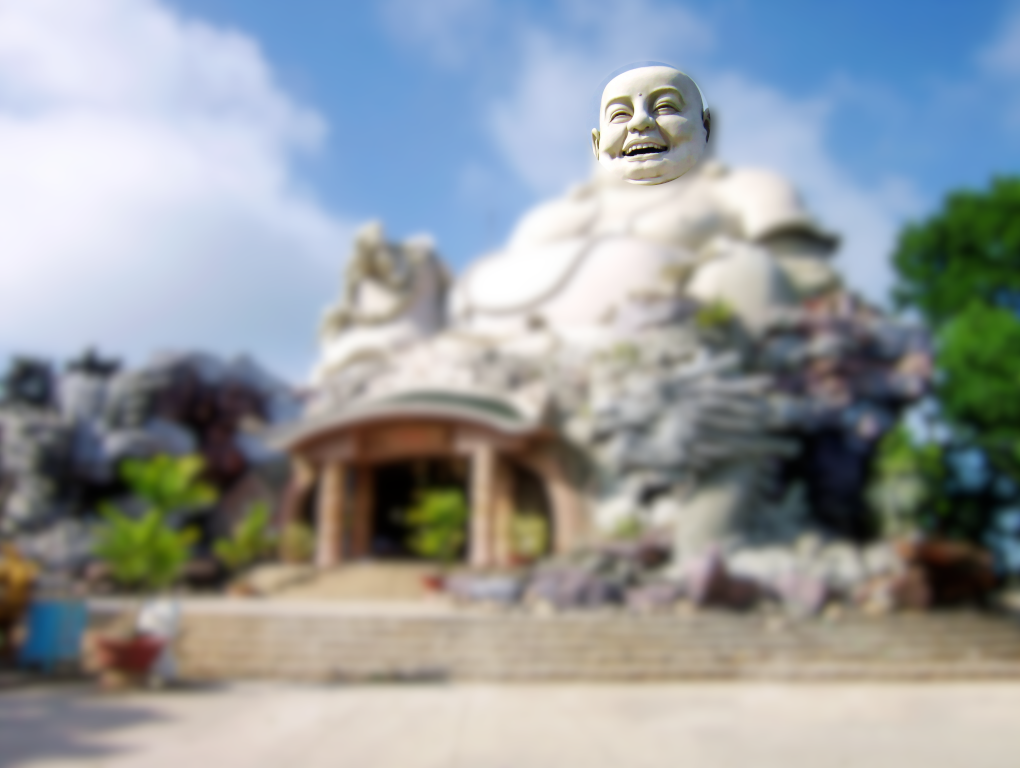
\includegraphics[width=\textwidth,height=\textheight,keepaspectratio]{logos/FoveatedImage.png}
     \caption{Foveated Rendered Image, picture originally from the DIVK dataset \parencite{Agustsson2017}.}
    \label{fig:foveated-rendering}
\end{figure*}

\par
One method to tackle the problem with the necessary quality level is to use foveated rendering. Initially, foveated rendering is used in the gaming area to increase quality while keeping high frames per second, and without it there would be curtailments in quality or FPS. The foveated rendering simulates the human’s view which is separated into two regions. The first is the foveal region, which is approximately 5$^{\circ}$ of the visual sight, is in the centre of the current gaze and is responsible for a sharp view \parencite{Yanoff2020}. The remaining view is grouped to the peripheral region and is less sharp and clear compared to the foveal region \parencite{Yanoff2020}. This fact leads to computing an image which has high resolution and full details at the current gaze while the background displays only contours of objects and is blurry. For example, see \autoref{fig:foveated-rendering} in which the head of the buddha statue is sharp, and the rest becomes blurrier. One requirement for this method is that the gaze’s current location can be determined in the image, which requires modern \gls{vr} glasses like the HTC VIVE Pro Eye \parencite{HTCVIVEProEye2020} or additional separate hardware like the Tobii Eye Tracker \parencite{TobiiTracker2020}. For streaming, foveated renering reduces the needed bandwidth while keeping good quality and reducing the latency.
\par
Another method for solving the streaming problem is to use \gls{ml}. With the increase of available hardware power, \gls{ml} is becoming more available for developers and users through consumer hardware. For streaming, the compression and decompression data are necessary steps and are typical for autoencoders. The problem with autoencoders is that they learn how to compress and decompress detailed data, and the outcome is restricted to this (training) material, whereas it needs to work with any unknown data. A different approach is to increase the quality of images after the transmission. For enhancing the quality of videos or images, \gls{sr} is a promising method as it is a set of methods that reduce image noise and deblur. One of the newest and most suitable working methods is a \gls{gan} which is a deep convolutional neural network. Developed in 2014 by \citeauthor{Goodfellow2014}, \gls{gan} was first used to generate new images from random noise, for example handwritten numbers. Later on, it developed to a promising \gls{sr} method, with a low-resolution input and a high-resolution output. A prominent example is the \gls{srgan}, which is capable of generating realistic single textures \parencite{Ledig2017}. With DeepFovea, Facebook’s research lab tackled the problem of enhancing video sequences with \gls{gan} \parencite{Kaplanyan2019}. The original idea of DeepFovea was to enhance foveated rendered videos for \gls{vr} and to reduce the needed hardware power by reducing the resolution and restoring the background while keeping the foveal area in original high-density resolution.
\par
In conclusion, a stable streaming solution is required for telepresence that delivers a high-resolution video within a limited latency independently of the network conditions. The goal of this thesis is to build a streaming solution of 3D video data from one computer to another. On the receiver side, a \gls{hmd} is connected and displays the environment of the robot. The following steps were implemented: On the robot’s side called server, a camera is attached to record the environment. The camera stream is split into two parts. The first one is a high-resolution uncompressed video of the foveal area and the second one is a low-resolution compressed video of the peripheral area. For generating the foveal area, the server receives the current gaze of the user sequentially from the client. After both images are generated, and the peripheral region got compressed based on the available bandwidth, they are transmitted to the client. The client, where the \gls{hmd} is connected to, receives both streams and merges them according to the prior sent gaze coordinates. If necessary, the client performs SR of the peripheral region to achieve an overall good video quality. The resulting image is displayed in VR. For the next image, the client sends the \glspl{hmd} current predicted gaze to the server. The maximum latency from the robot to the user should be below 125 milliseconds.
\par
In order to achieve this goal, \autoref{chapter:background} introduces the current state of the art and the background of the used technologies to get a better understanding of the implementation. For a better comparison of the measuring, between different applications, \autoref{chapter:environment} introduces the used hard- and software. Chapter \ref{chapter:implementation} describes the implementation of low-latency streaming with foveated rendering and superresolution. The measured results of the formerly described implementation are presented in \autoref{chapter:evaluation}. Last but not least, \autoref{chapter:conclusion} outlines the conclusion and identifies the limitations. Finally, \autoref{chapter:outlook} gives a brief outlook for the next steps.
% !TeX root = ../main.tex
% Add the above to each chapter to make compiling the PDF easier in some editors.

\chapter{Background and Related Work}\label{chapter:background}
This chapter briefly introduces the related topics of this thesis. The main topics are streaming, \gls{vr} and \gls{sr}.

\section{Streaming}\label{section:background_streaming}
Streaming includes technology that transmits video sequences over the Internet \parencite{Mok2011}. Today, streaming is a billion-dollar business dominated by global players like Amazon and Netflix \parencite{AMR2019} Moreover, for live events in sports, eSport and more, streaming is becoming essential \parencite{AMR2019}. Viewing television online is also becoming increasingly more popular as cable TV is becoming less common \parencite{CableTV}. 
\par
The technical aspects of streaming include multiple steps. For streaming normal movies or series, the data is encoded into a specific format or multiple formats independent of the user’s device, as each device can handles different codecs. For example Android can handle encoding and decoding H.263 up to H.265, VP8 and VP9, wheres AV1 can only be decoded and only on Smartphones having the Android 10 or greater \parencite{Android2020}. Some codecs were mentioned before, like the H.265 or VP9. Although the codecs differ in how they compute the compression and decompression, they have commonalities. For example, the different types of frames exist to deliver the best possible image. The intra-coded frame (I-frame) is a complete image. The predicted frame (P-frame) contains changes between the I-frames. When there are moving objects in a scene with a static background, only the moving object has to be encoded to save bandwidth. The third and last type is the bidirectional predictive frame (B-frame), which saves more bandwidth by calculating the difference by future, current and past frames \parencite{Katto1995}. The computation of these different types is called encoding. After the encoding, the video is transmitted through a network to the user’s device, where the different frames are merged, which is called decoding. Most modern hardware supports the decoding. Otherwise, a software decoder is required, which is less efficient than the hardware. The encoding and decoding are necessary to achieve an acceptable quality of the video. The lower or more unstable that the connection from the server to the client is, the higher the computation. Since users want stable, high-quality streaming, considerable efforts are required to meet this demand. For a stream having resolution below 720p, is non-stop buffering or is pixelated is not accepted by the user \parencite{VideoAcceptance}. Most video providers perform pre-encoding of the videos in different resolutions and codecs to be used by different kinds of user devices. Pre-encoding saves computation time, resources and money, because performing the videos’ analysis and math beforehand reduces the hardware load at delivery as the encoding is performed once. Furthermore, no action by the user of the system is involved \parencite{Netflix2015}.
\par
However, low latency is vital for streaming live public events for viewers to see the action and react at an appropriate time and with other viewers simultaneously. Alternatively, the viewer cannot receive what the commentator has to say in a timely manner with respect to the streamed event. The created lag impacts the viewing experience negatively.
Additionally, live events from private persons are becoming more popular. With YouTube, Facebook and Twitch, some popular platforms provide a free possibility to interact with hundreds of viewers at the same time. Low latency is required not to lose the ov erview, as the presenter directly interacts with his audience.
\par
The difference between regular and live streaming is that the video of the former does not exist in advance. The video cannot pre-encoded. Performing the encoding on-demand leads to a higher overall transmission time. To reduce the delay, the B-frames or the P-frames are disabled, as their computation is challenging and needs time. The remaining I-frames are whole images, which leads to a high bandwidth \parencite{Katto1995}. Typically, the live streams are not shared directly between the broadcaster and the spectators. Instead, between these two entities is a streaming distributor with more bandwidth capabilities than normal users have at home. The broadcaster uploads his video stream to the distributor, which shares the stream with the broadcasters’ viewers, as the broadcasters bandwidth capacity is limited and cannot handle many viewers. Examples of streaming distributors include YouTube \parencite{Youtube} or Twitch \parencite{Twitch}, which offer a complete platform with a full-service package. Moreover, other business-oriented delivery networks such as \cite{Akamai2020} exist. When latency is critical, a one-to-one connection is necessary to avoid all possible disturbances.

\section{Virtual Reality}\label{section:background_virtualreality}
The idea behind \gls{vr} was created in 1965 by \citeauthor{Sutherland195} with the title 'The Ultimate Display'. However, the first system able to show a virtual scene was created in 1962 by \citeauthor{Heilig1962} and was called Sensorama. Many iterations later, \gls{vr} is becoming applicable and affordable for many developers and users. For example, IKEA allows its customers to create virtual kitchens to inspect how their new kitchen would look like \parencite{Ikea2020}. Furthermore, the car manufacturer Audi shows a potential new car with all its possible configurations in a manner that is as realistic as possible for customers to have a better feeling of how the new car appears \parencite{Audi2017}. Moreover, in the medical sector, \gls{vr} is used to relieve amputees' phantom pain by controlling a virtual body part. Performing the movements is done by recording the electrical signals of the damaged limb \parencite{Murray2007}. All \glspl{hmd} displaying the virtual reality consists of two small screens directly in front of the user's eyes. In front of these screens are fish-eye lenses to create a spherical panorama. Both screens show the same content. Different techniques are used to create a steroscopic effent. One of them is to slightly shift the content horizontally on each screen presenting a different view of the scene to each eye. Moreover, other depth cues such as parallax, where objects in the distance move slower than the objects close up. Also lenses are used , where barrel distortion provides an enourmous field of fiew (FOV). These methods lead to an immersive 3D feeling for the user. 
\par
Aside from the stereoscopic effect or the design of the graphics, other factors impact whether the user thinks the virtual environment is realistic. Tracking the motion of the headset is essential to cultivate an immersive feeling. When the user rotates their head or moves, visualising the motion is essential. For example if the user rotates its head by a certain angle, the virtual view should rotate by the same angle. Some papers mention 11 milliseconds latency between the motion and the image refresh. Otherwise, a lack of realism due to motion sickness exists \parencite{Kim2018}. This notion 'refers to the illusion that the scenario being depicted is actually occurring' \parencite{Slater2009}, which means that the user feels that what is happening is real.


\begin{figure*}[t]
    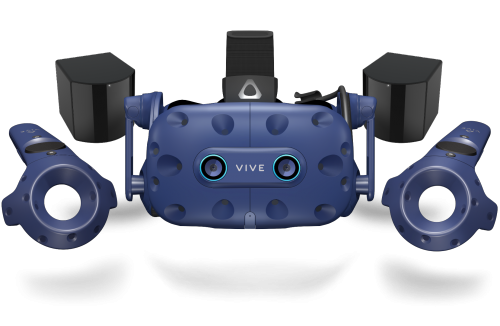
\includegraphics[width=\textwidth,height=\textheight,keepaspectratio]{logos/viveproeye.png}
     \caption{HTC VIVE Pro Eye, a \acrshort{vr} headset with controllers and tracking, image taken from \cite{HTCVIVEProEye2020}}
    \label{fig:htcviveproeye}
\end{figure*}

\section{Foveated Rendering}\label{section:background_foveatedrendering}

Foveated rendering is a new method of reducing the workload required for \gls{vr}. It was first mentioned in 2014 by FOVE, who invented the first head-mounted display with integrated eye-tracking to calculate foveated images based on the current gaze. With foveated rendering, the workload is lessened by reducing the image quality outside of the foveal area. As mentioned before, the foveal region is one of two regions of humans' vision. Foveated rendering recently reached consumer hardware, in particular through the VIVE Eye Pro \parencite{HTCVIVEProEye2020}, whereas a competitor, namely the Oculus Quest \parencite{Quest2020} supports a low-level implementation of foveated rendering called \gls{ffr} because of the lack of eye-tracking. \glsfirst{ffr} assumes a gaze more or less in the centre of the image. The developers set the hardness of the reduced quality in different steps. Foveated rendering's purpose is to reduce the number of pixels within the peripheral area. During runtime, the image is filled with interpolated pixels to achieve the desired size. Aside from reducing the workload by decreasing the calculated amount of pixels, foveated rendering also reduces the needed bandwidth as the image's size is reduced. To return the image to its original size, using \gls{sr} is an acceptable method.
\par
Foveated rendering is not only used for \gls{vr} gaming to lower the hardware. \citeauthor{Illahi2020} describe a method of how foveated rendering is also suitable for cloud gaming. In cloud gaming, the game is rendered through a server and streamed to the user. Simultaneously, the users' input is sent to the server so that on any device any game is playable independent of the users' hardware. In the paper by \citeauthor{Illahi2020}, the gaze is used for calculating a custom discrete cosine transformation (DCT) for the H.264 codec. In this codec, the image consists of pixel partitions from 16x16 to 2x2, but 8x8 blocks are primarily used. The block is processed by the DCT followed by a quantisation which requires a quantisation step \(Q_{step}\), which is precalculated and is applicable for all dimensions that are divided by eight. The paper proposes an offset for this \(Q_{step}\) bases on the current gaze, resulting in a foveated rendering where the more distant parts are more quantised and therefore have lower quality. 
\par
Furthermore, \citeauthor{Guenter2016} discuss how 360$^{\circ}$ videos are streamed with the technique of foveated rendering. They propose dividing an image into tiles and having smaller horizontal regions at the top and bottom and larger tiles in the middle as they are more in the users' view. Streaming each tile in low-resolution separately results in low bandwidth and reduces the computational need. The exception is when the tile is active, such as when the user actively looks into this tile, and then the tile is streamed in high-resolution. This technique allows efficient streaming of 360$^{\circ}$ videos without losing details, and having a sharp image in the users' gaze. 


\section{Superresolution}\label{section:background_superresolution}
A variety of image enhancement tools exist, including professional software like Adobe Photoshop \parencite{Adobe2020} as well as open-source projects like GIMP \parencite{Gimp2020}. These tools allow manual adjustments for better details, contrast and more. They also include tools to enhance a full image, for example deblurring a photo with the Wiener Filter \parencite{Wiener1964}. Using these tools requires experience, because blurring or other quality-weakening details need to be detected. For this reason, researching automatic image enhancements has become of interest to users, and new applications like video stream enhancements have become possible. One of them is \gls{sr}, which increases the size as well as enhances the quality.
\par
\Acrlong{sr} is a modern technique to enhance images. Improving images is necessary for multiple reasons, such as increasing the size if an image has a smaller spatial resolution than it should have. Another scenario is to have more details at specific regions, for example for cancer detection in an MRI scan by zooming into one region \parencite{Chaudhari2018}. The most general case is to have a beautiful image. Thus, analysing incoming images to determine the best possible options is essential, because the exact degradation function, is unknown. This function stores the information about defects such as blur and noise. Low-quality images are improved to good quality, and enhancing the images with good quality leads to more details by estimating them where they are unknown. Moreover, \gls{sr} reduces noise and blur in many cases. Performing the \gls{sr} in real-time is also necessary for some applications, such as live streaming or gaming. Simple methods perform the upscaling by interpolating nearby pixels to increase the overall number of pixels. However, related to the increasing attention given to movies, films or other moving images as well as the interest in better image quality, the research in \gls{sr} is making considerable progress.
\begin{figure*}[htbp]
    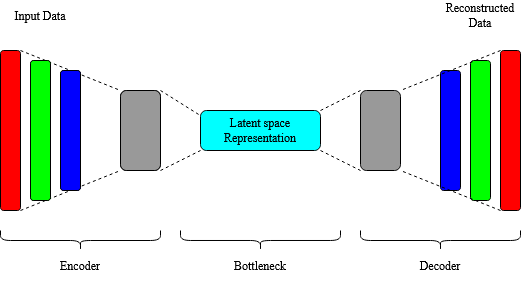
\includegraphics[width=\textwidth,height=\textheight,keepaspectratio]{logos/Autoencoder.png}
     \caption{Autoencoder}
    \label{fig:autoencoder}
\end{figure*}

\par
With \gls{dlss}, Nvidia launched one of the best-known \gls{sr} examples \parencite{DLSS2020}. It is capable of real-time \gls{sr} of 3D games. For this purpose, a deep convolutional neural network has an input of a low-resolution image as well as a motion vector which are both generated by the game engine. \gls{dlss} generates an image, which has a resolution one step higher. A step higher means that 540p input images have a 1080p or Full HD output image, whereas \gls{whqd} = 2560x1440 pixels images have a 4K resolution as an outcome. For their \gls{sr}, Nvidia used an architecture called convolutional autoencoder. The generated images were compared against 16K reference images, which resulted in a difference map which was forwarded back into the neural net to improve the results further. The remarkable aspect is that not every game is trained separately, as the network is trained generically and thus fits to a wide range of games. The original background of autoencoders is to learn efficient data representation. An autoencoder consists of an encoder making the data as dense as possible, most likely by dimensionality reduction. In \autoref{fig:autoencoder} the data has to be represented in such a manner that it fits through the bottleneck. On the other side of the bottleneck, there is a decoder with the goal to reconstruct the data by minimising the reconstruction error. Both the encoder and decoder are neural networks, typically with one hidden layer. Otherwise, the autoencoder is called deep autoencoder. There are the following two types of encoding:
\[x \neq d(e(x)) \]
whereas \(x\) represents the data, \(d(x)\) the decoding and \(e(x)\) the encoding.
The first equation represents the more probable situation, being the lossy encoding, where information is lost. In this subject, lossy means that the data cannot be fully restored after the compression. The other equation
\[x = d(e(x)) \]
represents the lossless encoding meaning that no data in the decoding is lost. As its only goal is to dense data, it is not capable of handling new data or even generating new data.

\par
\Acrlong{vae} where 'variational' comes from the variational inference, are one new step further and are capable of generating data. The \gls{vae} ensures that its latent space has good properties by regularising the distribution during training to generate new data. More specifically, it learns a latent variable model, which means it learns the parameters of a probability distribution which represents data instead of learning the data itself. It does not turn a sample into a parameter. Instead, it uses the mean \(\mu\) and the standard deviation \(\sigma\) of the data which are assumed. The stochastic encoding means that even for the same input, the actual encoding varies on every generation, which leads to a decoder having as input not only specific data points as generated by the standard autoencoder but also slightly varying encodings which cannot be differentiated. Thus, the \gls{vae} is capable of generating new data that looks similar to the existing material which can be generated randomly as well as in a specific direction. Additionally, as the range of \(\mu\) and \(\sigma\) are infinitely broad, the encoder has to learn these different values and ensure that it does not significantly vary from the same input. This behaviour allows the decoder to reconstruct the training data efficiently. Although the quality of the reconstruction and the desired outcome is dependent on the neural network that is used, it is a useful method for enhancing images. Variational autoencoders are one type of generative model, and another type are \glspl{gan}.

\begin{figure*}[htbp!]
    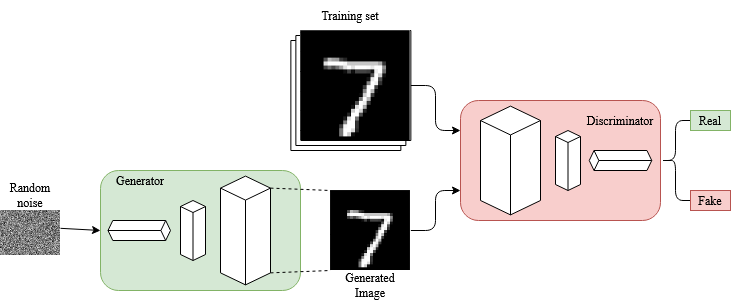
\includegraphics[width=\textwidth,height=\textheight,keepaspectratio]{logos/GANSchematic.png}
     \caption{Example of \acrshort{gan} as proposed by \cite{Goodfellow2014}}
    \label{fig:ganfigure}
\end{figure*}

\par
This type of neural network was initially developed to generate new images. It consists of two neural networks, a generator and a discriminator, that work against each other. The final goal is that a generator creates new images through random noise input. The training consists of the neural networks. The discriminator receives the images generated from both the generator and the training set as input and has to learn to differentiate them. The generator receives input of random noise as training and learns to generate images which look similar to the ones in the training set. The loss function of the generator is the result of the discriminator whether the image got accepted or not. An example of this outcome is presented in \autoref{fig:ganfigure}, where the well-known \gls{mnist} dataset is used \parencite{lecun2010}, which contains thousands of handwritten digits. In this example, the generator tries to generate a number which is accepted by the discriminator. Aside from having noise as the input, a further step is to use other images as input that contain small structures. Images of a semantic object can be used in Pix2Pix networks to generate a complete image of them, for example generating an image of a complete house from a drawn building \parencite{isola2018}. This process also permits characteristic features of images to be mixed, which is enabled by a CycleGAN where for example, adding the stripes of a zebra to a horse \parencite{zhu2020}. A CygleGAN enables to train neural networks to translate an image to a target domain without paired examples, i.e. the target image is newley created without an ideal image. Increasing a smaller image in size without losing details is difficult even for modern techniques. Another well-working example for \gls{sr} is the \glsfirst{srgan} proposed by \cite{Ledig2017} which is built upon a \gls{gan}. The goal of \gls{srgan} is to learn the statistics behind a high-resolution image of a training set and determine how to get there from the lower resolution image. In comparison to the \gls{vae}, the learning process is different, and in a \gls{gan} another neural network decides whether the generated image is satisfactory. As the generator and discriminator work against each other, an equilibrium between these two achieves the best results. Alternatively, \gls{vae} maximises the lower bound of the log-likelihood. Therefore, \gls{vae} is more comfortable to train, as training only one network is necessary, which is in contrast to the training of two networks with \gls{gan} and keeping them both equal. As an example, \autoref{fig:srexample} demonstrates the differences between the \gls{srgan} generated image, the low-resolution input and the original high-resolution image. However, the generator does not necessarily have to increase the image size, as the other implementations have shown.

\begin{figure*}[t]
    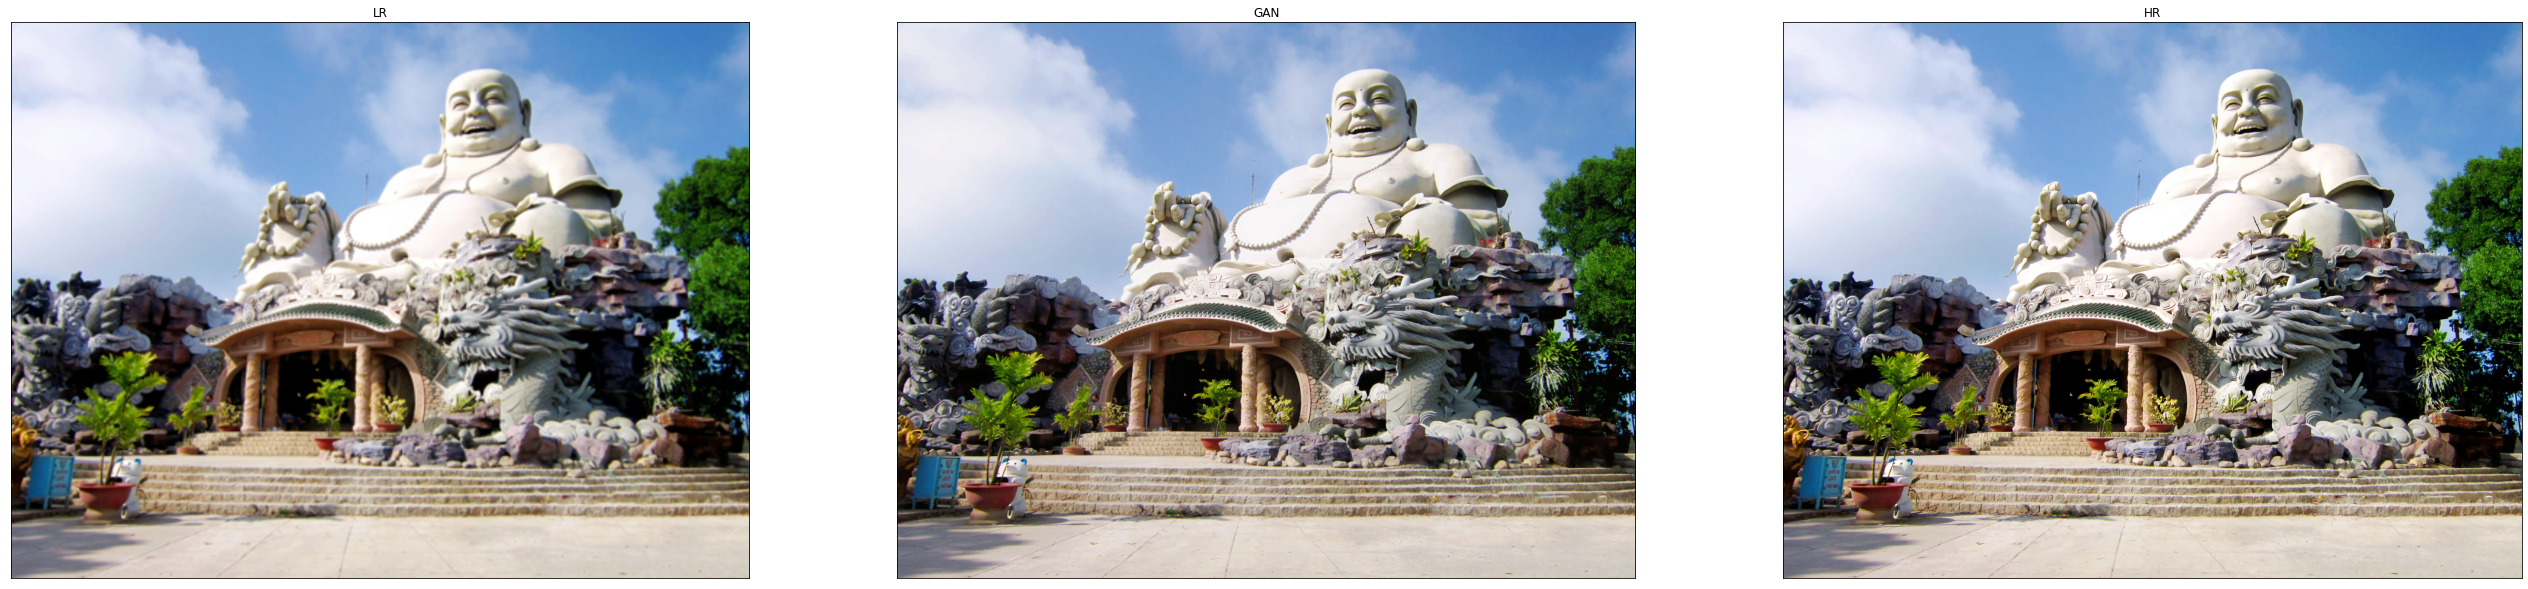
\includegraphics[width=\textwidth,height=\textheight,keepaspectratio]{logos/SR.png}
     \caption{Example of \gls{sr} as proposed by \cite{Ledig2017} with an example image from the DIVK dataset \parencite{Agustsson2017} }
    \label{fig:srexample}
\end{figure*}

\par	
In conclusion, multiple possibilities exist to generate new images out of existing images to add details, to compress them without losing details or to mix features. The presented two solutions namely the \gls{vae} and the \gls{gan} are the most promising ones as they achieve the best results. 


\chapter{Environment}\label{chapter:environment}
Before the state of the art technologies are implemented, which were presented in the last chapter. Describing the hardware and software for comparison provides a foundation for this thesis, since \gls{vr}, as well as real-time streaming, are still challenging for modern hardware,

\section{Hardware}\label{section:hardware}
Not many state-of-the-art head-mounted display with integrated eye-tracking exits. These are namely the HTC VIVE Pro Eye (see \autoref{fig:htcviveproeye}) or VRgineers’ XTAL \parencite{XTAL2020}. The first one has existing plugins for game engines and is widely available, and it is presented in \autoref{chapter:implementation}. In contrast, the XTAL has some more features like automatic eye calibration, but the software was not correctly functioning at the time of this project. Thus, the Pro Eye is used for the development of this project.
\par
For a network, usually two computers are necessary, but only one with the required hardware was available. Intel Realsense cameras are connected to a computer, acting as the server, which also performs the encoding of the streams. Efficient encoding is a matter of hardware as pure software encoding is much slower than the hardware-supported equivalents. There are two possibilities to encode on hardware: separated specialised hardware encoders and graphic cards. The first option receives a video input signal, encodes it and transmits it to the desired destination. It is mostly specialised on one codec which does not allow using multiple codecs such as the Matrox's H.264 encoders \parencite{Matrox2020}. The other option is to use graphic cards that are capable of encoding and decoding multiple codecs. Nevertheless, as the encoding is less critical for manufacturers than decoding, only the newest codes can be decoded and not encoded like the AV1 \parencite{AO2020}, which has had no consumer hardware implementation two years after its development. There is also a difference between the manufacturers as their implementation is also a factor. Currently, Nvidia’s solution called \gls{nvenc} is the fastest in the graphic cards segment, which is proven by multiple tests like references done by the streaming software OBS \parencite{OBS2020} and by self-comparison of an available AMD 5700XT and Nvidia 2080Ti. The last one was selected for further development. To serve the \gls{gpu} with data, the AMD Ryzen 3900X was used as this \gls{cpu} offers many core capabilities.

\section{Software}\label{section:software}
As previously mentioned, HTC offers \glspl{sdk} for multiple game engines like Unity3D \parencite{Unity2020} and the Unreal Engine \parencite{Unreal2020} to use display footage and to track the eyes. Since both engines are powerful enough and capable of displaying a stream in \gls{vr}, there is no difference between them in this case. Unity3D was selected for personal preferences, and the version 2019.4 was used.
\par
Many streaming solutions exist that have a wide range of codecs implemented that are open source or professional solutions. As all of them include more or less the same codecs based more or less on the same implementation, and the availability of \gls{sdk} for the used software languages is essential as a C\# implementation is necessary for Unity3D. Thus, the open-source solutions FFmpeg and VLC are candidates as both have a satisfactory working command-line interface as well as available public \glspl{sdk}. Moreover, the implementation is different for web real-time communication or WebRTC, which is not a codec but a communication protocol and is based on HTML5 and JavaScript. As this is a protocol mostly made for real-time communication, it was added to the list of possible candidates. The results of the speed comparisons between the different codecs and WebRTC are in \autoref{chapter:implementation}.
\par
For the image manipulation at the server-side, i.e. resizing and cropping the python implementation of OpenCV is used because OpenCV contains \gls{gpu} optimimized algorithms. OpenCV is also used for catching the video stream from the camera and splitting the vidoe into single images.

% !TeX root = ../main.tex
% Add the above to each chapter to make compiling the PDF easier in some editors.

\chapter{Implementation}\label{chapter:implementation}
In this chapter, the implementation of the system will be discussed. The system contains multiple parts working in a continuous chain. Each member of the chain is discussed individually and is displayed schematically in \autoref{fig:fullsystem}.

\begin{figure*}[htbp]
    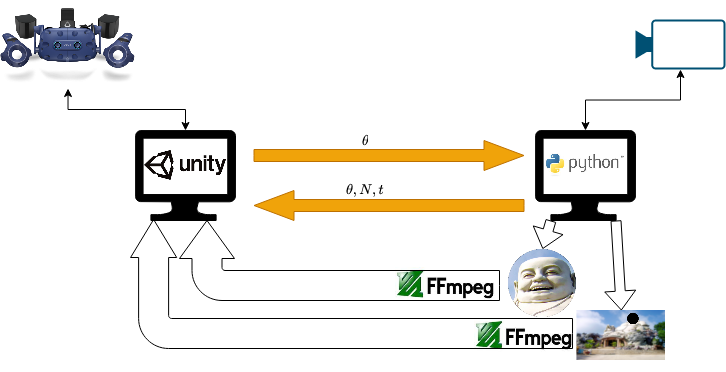
\includegraphics[width=\textwidth,height=\textheight,keepaspectratio]{logos/SystemSchematic.png}
     \caption{Schematic representation of the presented solution.}
    \label{fig:fullsystem}
\end{figure*}

\section{Foveated Streaming}\label{subsection:foveatedstreaming}
To create a foveated rendered image, locating the current gaze \(\theta\) is required. The \gls{sdk} SRanipal for the VIVE Eye Pro for Unity3D allows collecting the gaze in Unity’s update loop. The update method indicates every frame which results in a predicted \(\theta\) every 33ms when the \gls{vr} is running with 30 FPS or faster with a higher FPS. Furthermore, \(\theta\) does not correspond to the actual video coordinate system as it is guilty of the VIVEs’ system. Through RayCasting, Unity3D offers the possibility to isolate the position of a point in the view of the camera. The in-game camera calculates the hit point with a given direction, which is the current gaze. Additionally, the calculated position must be transformed to fit for the video. The predicted \(\theta\) is sent to the server through \gls{udp} as depicted \autoref{fig:fullsystem}.

 \par
In the server, a python instance runs which collects the stream of the cameras with OpenCV and crops the foveated area accordingly to the received gaze. Applying the idea of \citeauthor{Guenter2016} of streaming the images of the video as tiles instead of a complete frame, the foveated area and the peripheral area are streamed separately. FFmpeg starts with the following command and is filled with parameters explained later:
\begin{lstlisting}
    ffmpeg 
    -hwaccel cuvid 
    -y 
    -f rawvideo
    -vcodec rawvideo 
    -s  dimension 
    -pix_fmt bgr24  
    -I -
    -an 
    -vcodec hevc_nvenc 
    -maxrate speed_limit 
    -bufsize buf_size 
    -tune zerolatency 
    -pix_fmt yuv44p 
    -vsync passthrough
    -sdp_file sdp_file 
    -f rtp rtp:ip_adress:port
\end{lstlisting} 
\noindent
The command -hwaccel selects the hardware transcoder to fasten up the encoding or decoding, as it is different for each manufacturer and is in this case ‘cuvid’ to select Nvidias’ hardware transcoder . The next parameter -vcodec sets the input signal as it is unknown, because no file is given and is therefore not determined. It can be any codec like mp4, libx264 or rawvideo, meaning that it is not transcoded and is in width x height x colour-depth format. The command -s specifies the dimension of the input whereas -pix\_fmt specifies the colour format. The input given by the -I of FFmpeg is a raw image piped through the command line and thus does not exist in advance. The hyphen signals the piping. After this command, every other parameter sets the output. Since no sound exists, no sound is transmitted, which is given by -an. In addition to the specified input codec, the output codec also has to be specified. In this case, Nvidia’s Nvenc performs the H.265 encoding. Limiting the bandwidth in FFmpeg is possible with the command -maxrate. Using this command also requires using -bufsize, which controls the variability of the output bitrate. The command -tune zerolatency assures that a high encoding speed has the most importance to resume a lower quality. The YUV444p indicates the 4:4:4 chroma subsampling. The vsync parameter with the entry passthrough forces the encoder not to add interpolated images. This means that between two real frames there is no other frame added to reach a certain framerate, which is not counted correctly and therefore cannot be merged with the foveated region. The parameter -sdp\_file filename creates an sdp file stating the information about the stream and looks like the following example for an H.265 stream: 
\begin{minipage}{\linewidth}
\begin{lstlisting}
v=0
o=- 0 0 IN IP4 127.0.0.1
s=No Name
c=IN IP4 127.0.0.1
t=0 0
a=tool:libavformat 58.47.100
m=video 5004 RTP/AVP 96
b=AS:2000
a=rtpmap:96 H265/90000
\end{lstlisting}
\end{minipage}
Moreover, stated in the parameter list is the real-time transport protocol (RTP), which is a package-based protocol and is responsible for the continuous transmission of the data. The Internet Society defined it as RFC 3550 \parencite{Schulzrinne2003}. Using this protocol requires stating the sdp file as the input, specifieng the stream details.

\par
Since the predicted gaze is not 100 \% accurate, it slightly flickers even when the eye is not moving and there is a delay of the visible image, the selected foveated area is more significant than the mentioned 5$^\circ$ of the human’s view. Having an \(r = 128\) pixels resulting in a 256x256 image size worked well during the development. These images are streamed in full resolution with the highest possible quality as this is visible for the user. Oppositely, the peripheral area is compromised as much as possible without losing too many details to save bandwidth and to save computation time, as smaller images are easier to encode than larger ones. Therefore, the size of the background is reduced, resulting in a 512x256 image. This size is not precisely \(\frac{1}{4}\) of a 1920x1080 = Full HD image, and for the \gls{sr}, because the image should be dividable by 128. The resulting upscaled image is therefore 2048x1024 being in a 1:2 ratio instead of a 16:9 ratio. The reason this is necessary is explained in \autoref{subsection:superresolution}. An example of the possible result is presented in \autoref{fig:examplestream}. With the generated frame number, it is possible to connect the \(\theta\) coordinates to the frame, which becomes essential for merging both images. This step is necessary, because FFmpeg or VLC do not synchronise the frame count on the server and client side, as each side counts their frames from the beginning individually. Moreover, the coordinates cannot be parsed directly into the frame as the encoding process changes these values. The server sends the frame number, the coordinates and a timestamp as a package back to the client. This happens in parallel to the streams, as stated in \autoref{fig:fullsystem}.

\begin{figure}[htbp]%
    \centering
    \subfloat[\centering Foveated Image]{{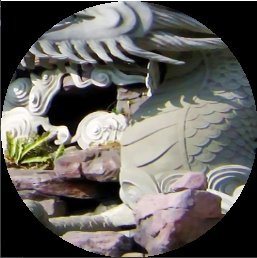
\includegraphics[width=2.56cm,keepaspectratio]{logos/FR.png}}}%
    \qquad
    \subfloat[\centering Peripheral Image]{{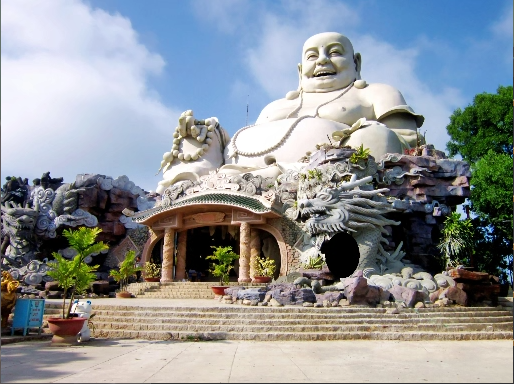
\includegraphics[width=5.12cm,keepaspectratio]{logos/peripheral.png} }}%
    \caption{Examples of the streamed images. The image is taken from the DIVK dataset \parencite{Agustsson2017}.}%
    \label{fig:examplestream}%
\end{figure}

\par
The server also tests the connection to the client to determine the available bandwidth \(\kappa\) at the beginning. This is possible since the iPerf3 is broadly available for different programming languages. This tool actively measures the maximum available bandwidth of networks. The measured bandwidth is divided by two and is the maximum available bandwidth for both the foveated and peripheral streams. The limit is inserted to the -maxrate parameter and in this scenario, the bufsize it set equal to the available bandwidth. 
\begin{center}
-maxrate \(\frac{\kappa}{2}\) -bufsize \(\frac{\kappa}{2}\)
\end{center}
\par
Back at the client-side, FFmpeg ist started with the command:
\begin{lstlisting}
    ffmpeg 
    -protocol_whitelist udp, rtp, file, pipe, crypto, data
    -hwaccel_output_format cuda 
    -probesize 32
    -analyzeduration 0
    -fflags nobuffer    
    -flags low_delay  
    -i sdp_file
    -vcodec rawvideo
    -pix_fmt bgr24
    -f image2pipe -
\end{lstlisting}
\noindent
The parameter -protocol\_whitelist is necessary for FFmpeg to use the stated protocols. The client incurs the hardware support parameter from the server as well as the flags for the low latency priority by signalling to avoid buffering and preferring a higher decoding speed. The probesize and analyzeduration parameters set the size and the duration of data which is analysed to obtain information from the stream. As this process adds some latency, it is reduced to the lowest possible value. The given sdp-file as input is generated by the server and is provided by using a weblink or by copying the file. The output of the decoding is images in the BGR colour scheme piped through the command line.
\par
The client receives both streams as well as the data package. The package contains the frame-number, the corresponding gaze coordinates and a timestamp. As the streams and data packages are not received simultaneously, synchronising the frame-number between the client and the server is required. To obtain the current number, the FPS from FFmpeg is collected, which indicates how long the decoding needs for a frame. With the received timestamp, the network delay \(\tau\) is calculated, resulting in the following formula:
\[\lambda = CurrentFrame - Offset = CurrentFrame - \frac{\tau}{\frac{1000ms}{FPS}} \]
\par
The algorithm stores the calculated frame number until FFmpeg decodes the corresponding frame. At this time, the peripheral area is resized to its original size, which is performed classically with a bicubic interpolation or \gls{sr}, and it is compared by quality and latency. Afterwards, OpenCV merges the foveated and the peripheral region at the corresponding coordinates. As the calculation is multithreaded, the merged images may appear in the wrong order, but as the processing takes more or less equally, it rarely happened during the development. That late processed images were shown to the user was prevented by checking the frame number. 

\begin{figure*}[htbp]
    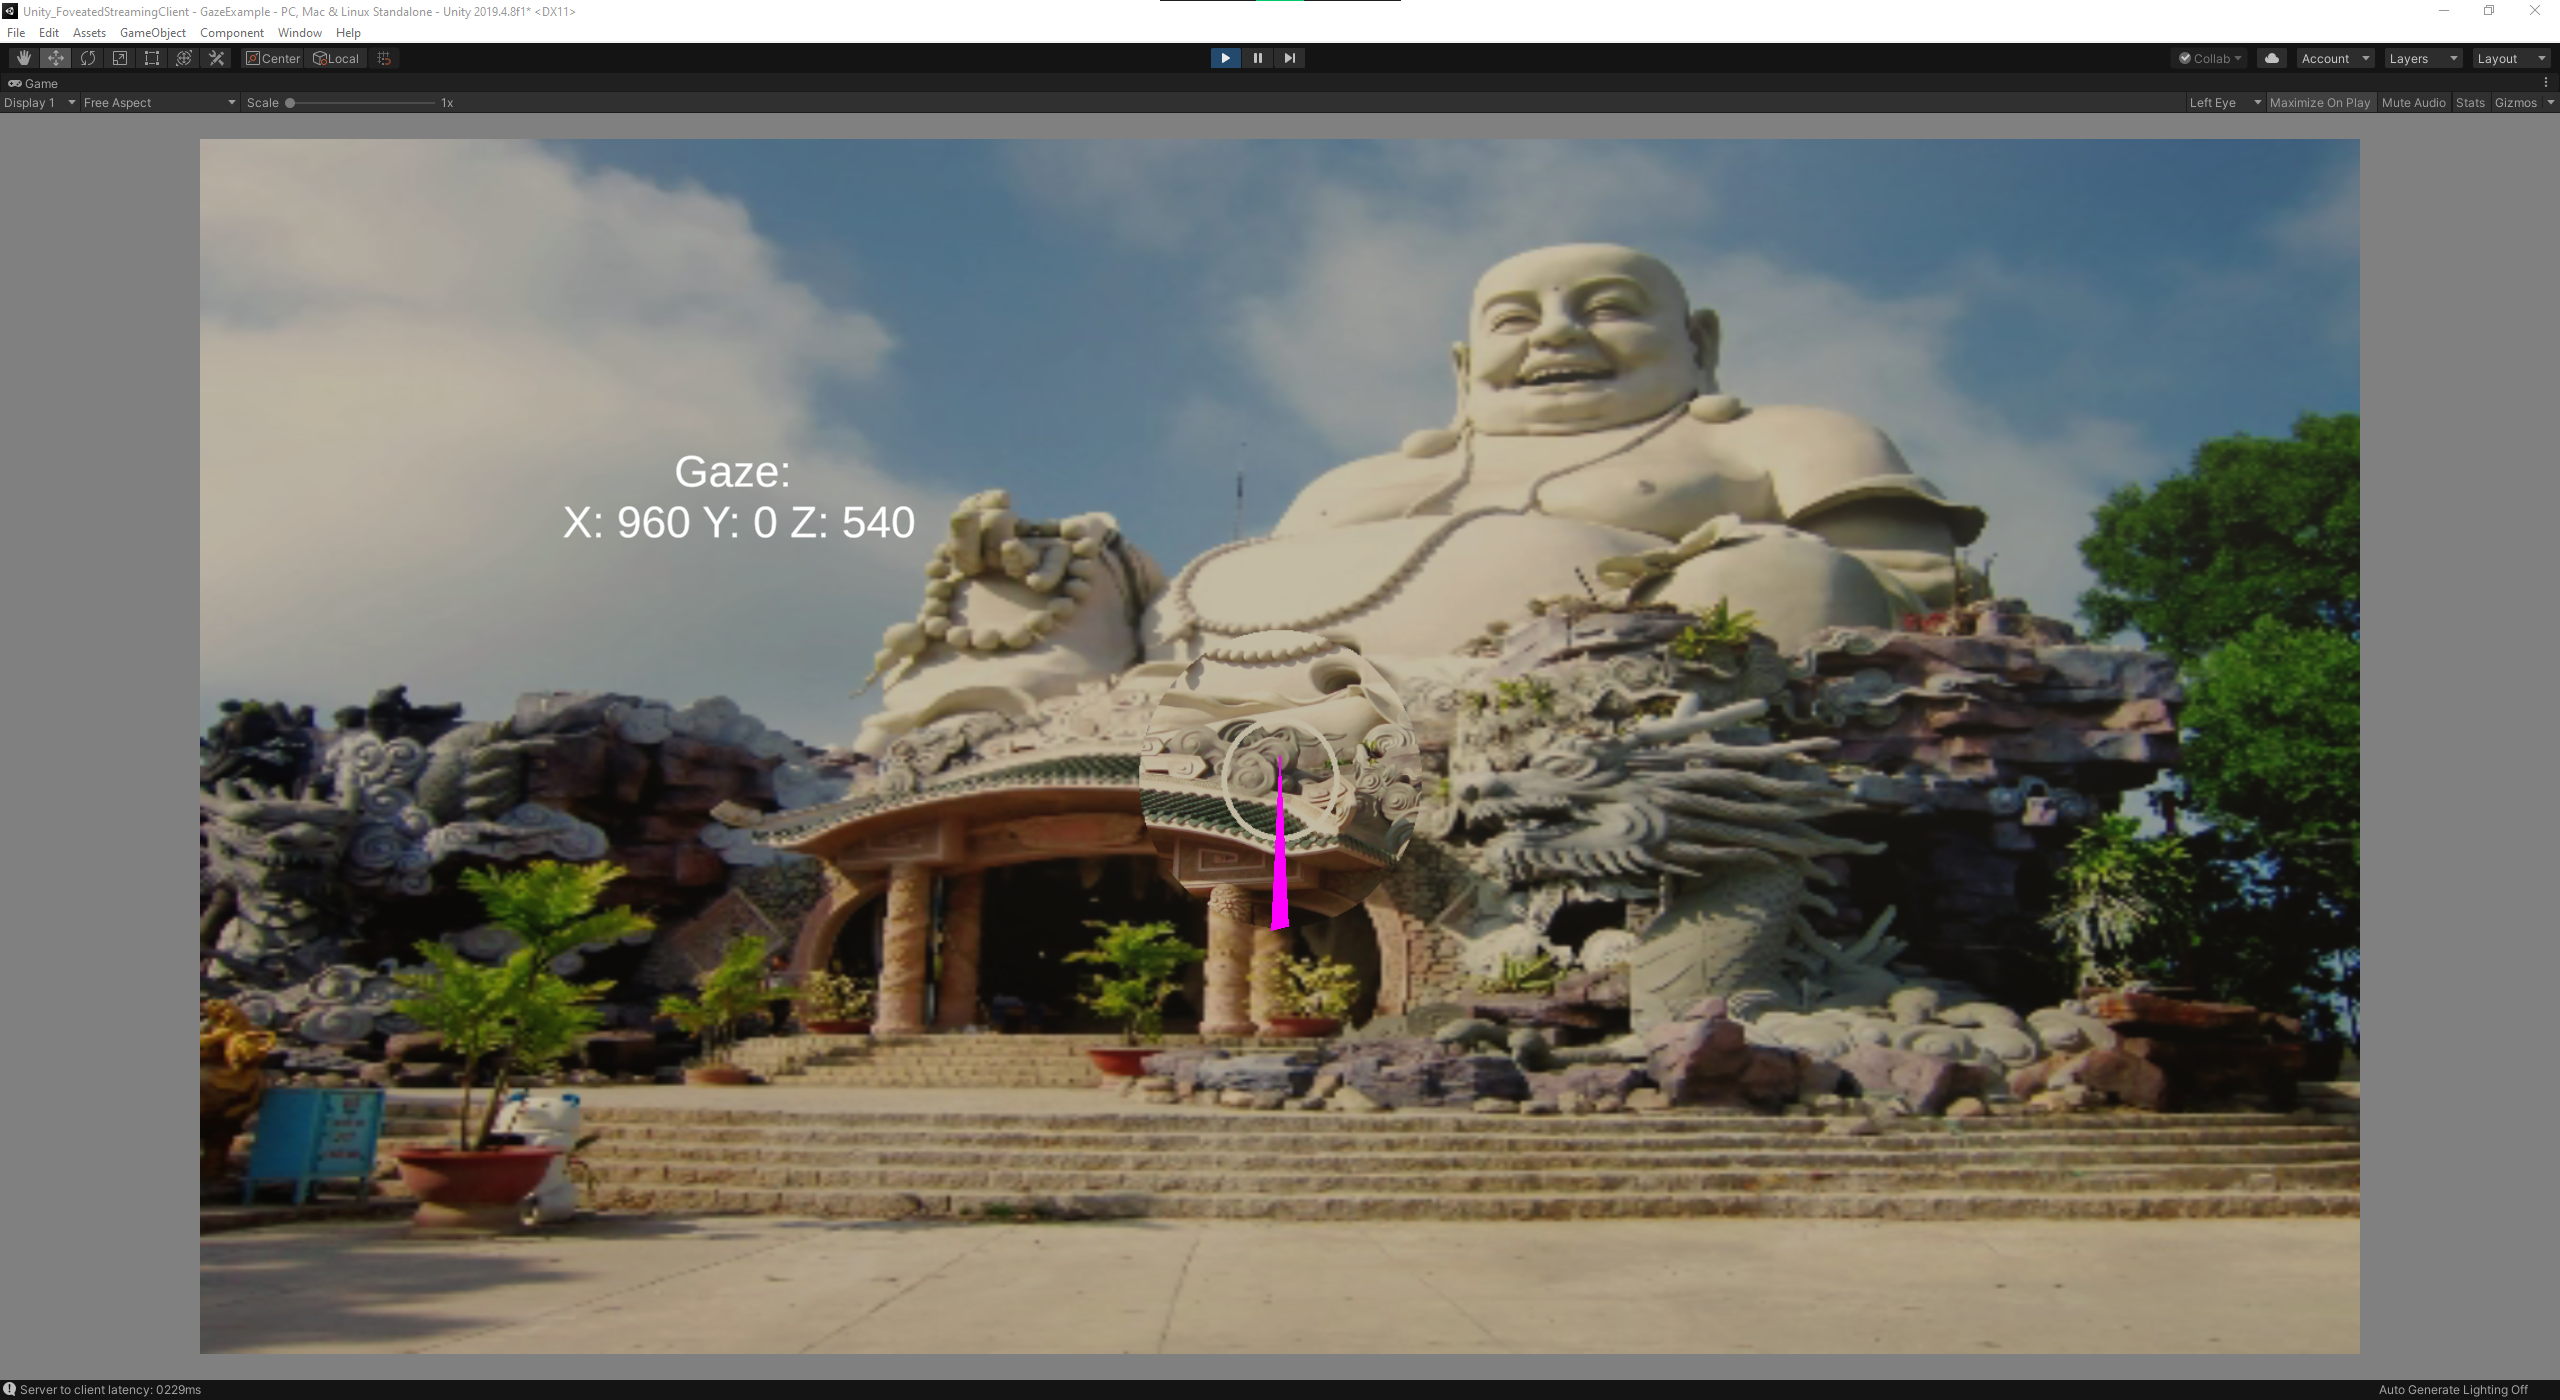
\includegraphics[width=\textwidth,height=\textheight,keepaspectratio]{logos/unity3d.png}
     \caption{Example view of a received image in 3D. The pink arrow displays the current gaze, whereas the white circle indicates the received gaze. The image is from the DIVK dataset \parencite{Agustsson2017}}
    \label{fig:unity3dgameview}
\end{figure*}

\section{Visualization}\label{subsection:visualization}
Unity3D displays the foveated rendered image on a plane in the 3D view. The result is visible in \autoref{fig:unity3dgameview}. Unity3D requires using a 3D object as a video screen, as the Raycast does not hit pure UI elements which would result in not having the correct coordinates. Additionally, the image is stretched as the image is mapped from a 3D game view to a 2D image.

\section{Superresolution}\label{subsection:superresolution}
To increase the size of an image, the missing pixels in between have to be calculated. Image libraries estimate these unknown pixels with different interpolation techniques such as the bicubic method, which uses 4x4 pixel squares to determine a new pixel by identifying the coefficients of the pixels in the square. This method is a considerable operation, and the nearest neighbour interpolation takes the average of the neighbours and is consequently faster. These methods work for each image individually, leading to recalculate the same pixels again and again when the image looks similar, as the algorithm has no memory about the preceding images. The example in \autoref{fig:comparison} shows that the bicubic interpolation has smoother edges than the liner one, but it is much weaker in terms of quality than the original high-resolution image. Another possibility is to use \gls{ml}-based \gls{sr}. \glsfirst{ml} has the advantage to learn the statistics of thousands of images. In this scenario, the focus is primarily on time rather than on quality, as the peripheral area is not in the user’s gaze and, therefore, is seen more schematically. Alternatively, when the available bandwidth is low, the pixelated image becomes visible for the user and should be avoided. Thus, the goal is to keep a minimum level of quality balanced with the latency. Facebook created with DeepFovea, which is a \gls{gan} capable of performing the \gls{sr} with four Nvidia Tesla V100 in under 10ms \parencite{Kaplanyan2019}. Additionally, it took less than 1ms to calculate a sparsified matrix of the current game view. However, this amount of graphic cards were not available. Moreover, calculating the 5D matrix as described in FaceBooks’ paper, is not usable as the image is streamed and decoded in the BGR colour scheme, which has only three dimensions. In contrast, the \gls{srgan} is capable of performing \gls{sr} with a good result but is slower as many more layers are used. Therefore, a mix of both of them is the right approach.


\begin{figure*}[htbp]
    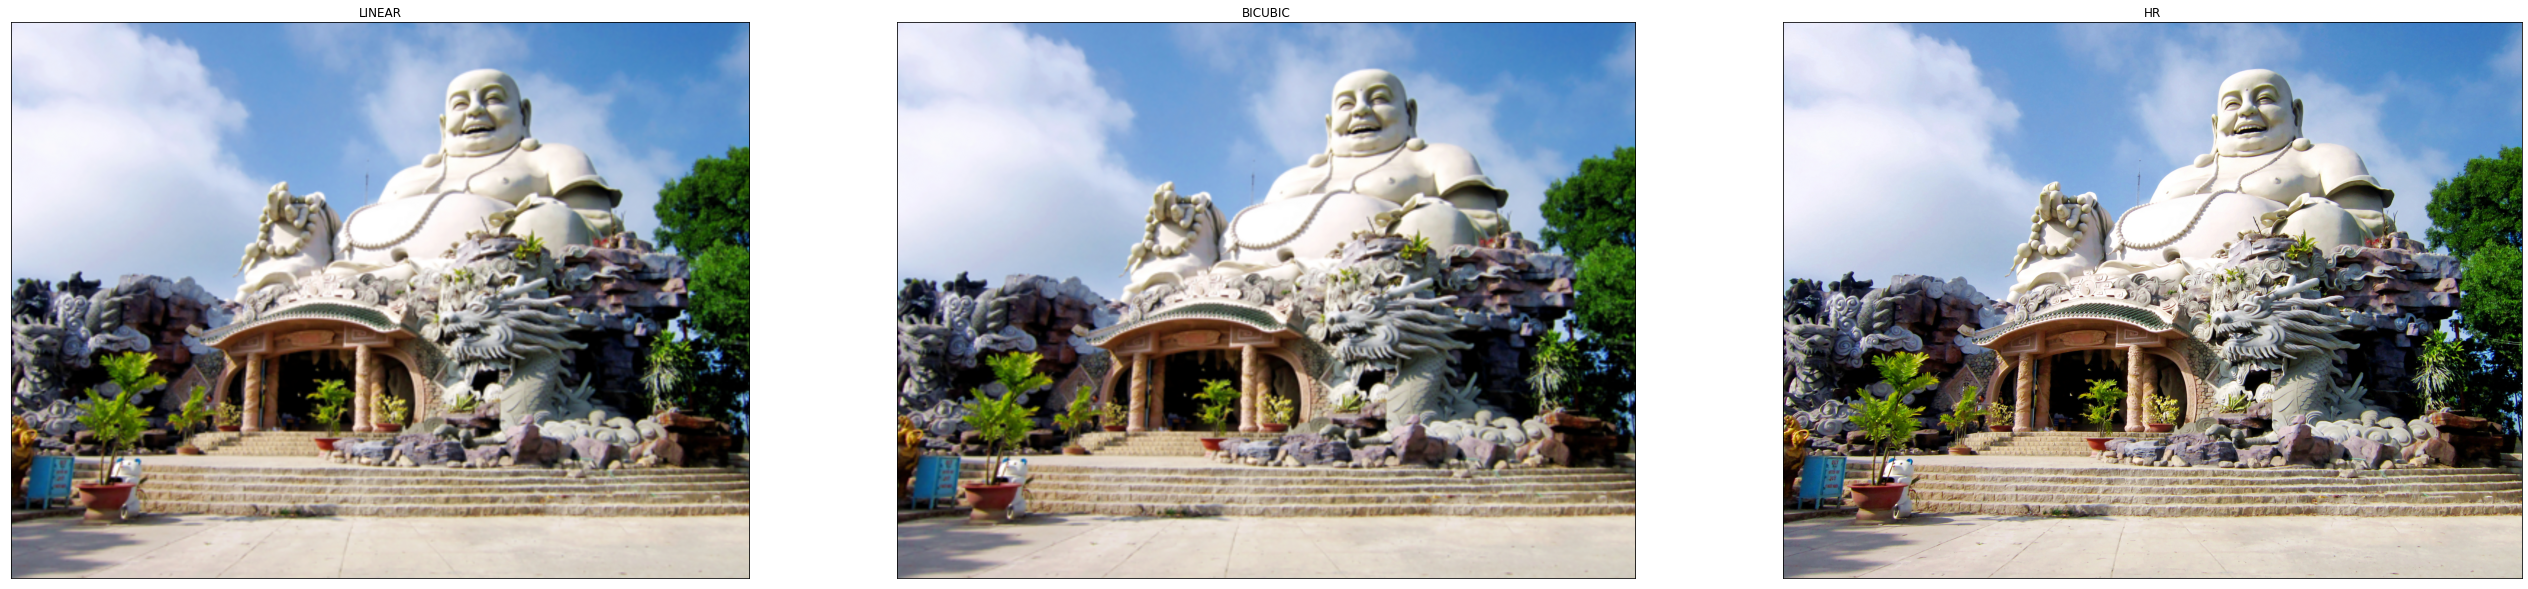
\includegraphics[width=\textwidth,height=\textheight,keepaspectratio]{logos/comparisonstandardresize.png}
     \caption{Comparison of the standard interpolation methods in comparison to the high-resolution image, which is taken from the DIVK dataset \parencite{Agustsson2017}}
    \label{fig:comparison}
\end{figure*}

\par
At first, a \gls{gan} consists of two neural networks: the generator \(G\) and the discriminator
\(D\). The goal of the discriminator is to differ between the training images and the images generated from \(G\). The images are classified as 1 or 0 by the discriminator. Classified as 1 means that the image seems to be real. This leads to a minimisation problem for \(D\) whereas \(G\) is a maximum likelihood function and therefore tries to maximise the objective function, which results in the following formula:

 \[ \min_{G} \max_{D} V(D,G)=\mathbb{E}_{x \sim p_{data}(x)}[log D(x)]+\mathbb{E}_{z \sim p_{z}(z)}[log(1- D(G(z)))] \]
 
The problem with the traditional function is that there is no automatic balance between the generator and the discriminator, and the balance has to be ensured by carefully performing the training. This problem is because the discriminator has a more straightforward job and is thus faster at learning, which results in an underperformance of the generator. This scenario leads to an unpredictable behaviour, and training the same model does not result in the same outcome, as seen in \autoref{fig:failedgan}, where the \gls{gan} reconstructs a given image in the wrong colour in one training. The problem was stated by \cite{salimans2016} that the models hardly achieve the Nash equilibrium, which states when two or more non-cooperative players in a game know each other’s strategy, the best option for each player is to change their strategy. Each model updates its cost individually, which leads to a possible divergence.

\begin{wrapfigure}{l}{0.5\textwidth}
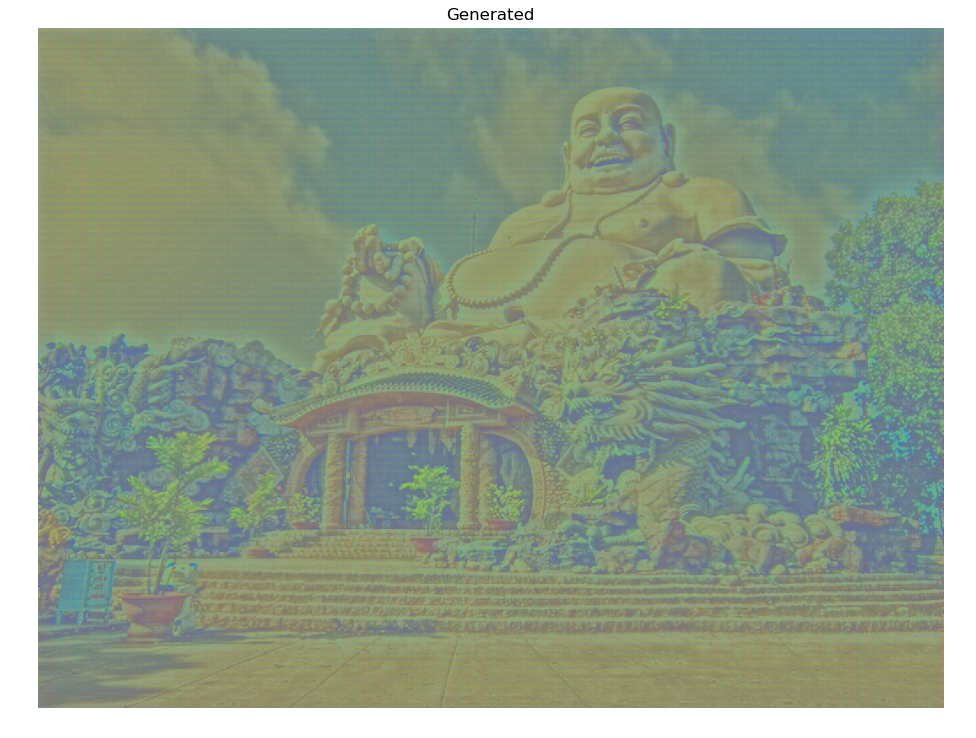
\includegraphics[width=0.9\linewidth]{logos/image_at_epoch_20000.png} 
\caption{Failed training of a \gls{gan}. Image is taken from the DIVK dataset \parencite{Agustsson2017}}
\label{fig:failedgan}
\end{wrapfigure}

\par
Researchers proposed many solutions to keep both in equilibrium. One paper by \cite{ham2020} proposes to pre-train the generator with a \gls{vae}. Since taking the trained weights from one model to a different model is not possible, the decoder of the \gls{vae} and the generator of the \gls{gan} are the same models. This pre-training results in preventing the \gls{gan} to collapse and increases the quality at early epochs. Another possibility is the WGAN named after the Wasserstein metric or Earth-Mover distance (EM distance) distance, which measures the distance between two probabilities \parencite{Vaserstein1969}. In this case, it measures the distance between the generated data distribution \(P_{g}\)and the real data distribution \(P_{r}\) and is defined as

\[W(\mathbb{P}_{r},\mathbb{P}_{g}) = \inf_{\gamma \in \pi(\mathbb{P}_{r},\mathbb{P}_{g})} \mathbb{E}_{(x,y)\sim\gamma}[||x-y||] \]

The WGAN uses this metric as a new loss function of the generator for having a smoother gradient to ensure that the generator learns. The Wasserstein metric works better than the \gls{js} or the \gls{kl}, which are used in a standard \gls{gan}. The \gls{js} is not differentiable at \(\theta\) and the \gls{kl} results in infinity if the two distributions are disjointed. Both algorithms measure the distance of probability distributions as well as the Wasserstein metric. In contrast, the Wasserstein metric gives a reasonable distance. Additionally, the WGAN clamps the weights to a fixed range on every gradient update and uses the RMSProp optimiser instead of the Adam optimiser. Facebook uses a Spectral Normalisation as an extension for the WGAN, which ensures 1-Lipschitz continuity. The spectral normalisation is a weight normalisation technique to stabilise the training of the discriminator \parencite{Miyato2018}. In addition to the adversarial loss, DeepFovea uses more losses like the \gls{lpips} as an extension to the perceptual loss
for detecting distortions and the optical flow loss for stimulating temporal consistency across frames, which results in the follow summary of losses \parencite{Kaplanyan2019}:

\[ L_G = w_{adv}*L_{adv}+w_{LPIPS}*L_{LPIPS}+w_{flow}*L_{flow} \]
\par
The \gls{srgan} project takes a slightly another approach by replacing the MSE content loss of a standard \gls{gan} by a feature extracting method from a pre-trained VGG network, where the name comes from the Visual Geometry Group (Visual Geometry Group 2020) who aim to use a perceptual loss containing two components: a content loss \(l^{SR}_{X}\)and an adversarial loss \(l^{SR}_{GEN}\). The former is usually a pixel-wise MSE loss but often lacks at high-frequency content which results in overly smooth textures \parencite{Ledig2017}. This paper proposes to replace the MSE loss by a VGG loss, which is based on the \gls{relu} activation layers of the pre-trained 19-layer VGG network \parencite{simonyan2015}. This network is a deep convolutional neural network containing 19 layers. It is pre-trained on more than one million images taken from the ImageNet database \parencite{Russakovsky2015} and classifies images into 1,000 object categories such as ‘mouse’, ‘lion’, ‘computer’, ‘TV’ and more. This network originated in the classifying area has thus learned a rich feature representation for a wide range of many images. The adversarial loss is the binary-cross entropy of the generated images classified as real images and the overall sum of generated images in the batch. This results in the following subsequent loss \parencite{Ledig2017}:
\[l^{SR} = l^{SR}_{X} + 0.01 * l^{SR}_{GEN}\]
\par
The overall structural layout of the \gls{srgan} and DeepFovea are different. The \gls{srgan} uses a \gls{resnet} structure as a basic layout. A \gls{resnet} normally consists of several homogeneous blocks containing a skip connection. The skip connection connects the input layer with the output layer in addition to the layers in between. This approach avoids the problem of vanishing gradients which occurs in some cases when the gradient is small enough that the corresponding weight does not change its value, and therefore, the networks stop continuing to learn. By adding the skip connection, the block reuses the activation from a previous layer. During training, this reused value is muted by the actual trained value. The \gls{srgan} uses 16 residual blocks containing two parts. In the first one, a convolutional kernel (Conv2D) layer is followed by batch normalisation and the activation function \gls{prelu}. The second part contains a second Conv2D followed by batch normalisation and the skip connection from the input. Another skip connection surrounds all residual blocks. The approach of the hull of the residual blocks follows a traditional \gls{gan} setup \parencite{Ledig2017}.
\par
In contrast, DeepFovea uses a U-Net setting, which contains a contracting and expansive path, which in this case is an encoder and decoder. This network is based on a fully convolutional network with the main idea to learn the feature mapping of an image and to make it more nuanced than a classic convolutional neural network. For this, the U-Net learns the feature mapping when converting an image into a vector and reuses the mapping to convert the vector back into an image. In this case the degration function is known, as the degration is perfomed in the contracting phase. Therefore, two phases exist that look like a U-shape. In the first phase, which prepares the data to pass through a bottleneck, the spatial information gets reduced, and the feature information increases, which is called the contracting phase. In the expansive phase, both pieces of information are combined, as each block gets the input of the former expansive block and the corresponding contracting block. This setup ensures that the correct feature mapping which has been learned is used for the reconstruction. This process requires that the amount of expansive block is the same as the contraction blocks \parencite{ronneberger2015}. Furthermore, DeepFovea uses four residual blocks for the contracting, one connecting residual block as the bottleneck and four temporal blocks in the expansive phase. Each residual block contains two 3D convolutional blocks followed by an \gls{elu} activation function. Similarly to the \gls{srgan}, the residual block uses a skip connection from the input to the average pooling. The temporal blocks contain again two 3D convolutions, where the first one is followed by layer normalisation, an \gls{elu} activation and recurrent connection to the input. The second Conv3D has an \gls{elu} activation again and is followed by a bilinear upsample. The temporal block also contains a skip connection from the input to the upsample layer. The input of this network is a 5D sparsified matrix that contains more information in the foveated area and less information the further away from this region. This input requires using the 3D convolutional layers. This fact makes it hard to reconstruct this neural network for this project, because in this setting, only a three-dimensional image exists as an input. Therefore, the \gls{srgan} was used as the ground structure.

\begin{figure*}
    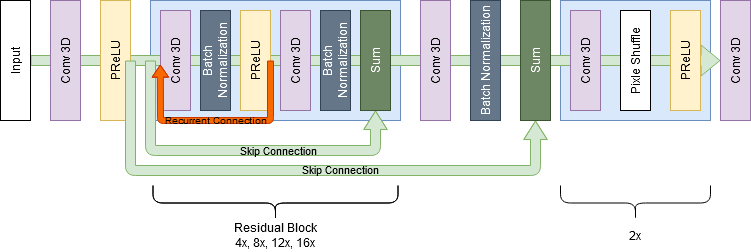
\includegraphics[width=\textwidth,height=\textheight,keepaspectratio]{logos/Generator.png}
     \caption{Generator}
    \label{fig:generator}
\end{figure*}

\par
As the generator from the \gls{srgan} works well in terms of producing quality images, the \gls{srgan} is taken as basis for further development. The first difference is inside a residual block where it becomes necessary to adjust the network from performing superresolution from images to videos. In this case, the idea of DeepFovea to use recurrent connections is implemented. Moreover, the more complicated and extensive a network is, the slower it becomes during live inference. Thus, the different configurations of the residual blocks are compared against each other. The generator is shown in \autoref{fig:generator}, with 4 to 16 possible residual blocks and the recurrent connection as an LSTM layer, which also requires to upgrade the Conv2D to a Conv3D as a dimension namely time is added. Alternatively, the training process and the loss function are different. First, the generator is pre-trained with an autoencoder as proposed by \cite{ham2020}. Second, the loss function is that of the DeepFovea’s as explained to comprehend the missing residual blocks. In particular, the neural network uses the combination of \gls{lpips} loss and optical flow loss in addition to the adversarial loss as proposed in the WGAN. The weights are the same as proposed by Facebook, namely: \(w_{adv}=1, w_{LPIPS}=100\). The optical flow had to be skipped due to hardware constraints. Additionally, the weights are clamped after each training process and the gradients are optimised by the RMSProp optimiser.
\par 
The discriminator has no impact on the latency, because it is not involved in the live inference and can be as large as needed. Therefore, the generators’ counterparty is the original from the \gls{srgan} with the improvements of the spectral normalisation. The resulting discriminator is presented in \autoref{fig:discriminator} \parencite{Ledig2017}.

\begin{figure*}[htbp]
    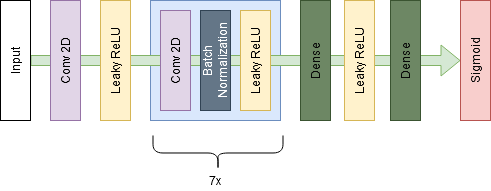
\includegraphics[width=\textwidth,height=\textheight,keepaspectratio]{logos/Discriminator.png}
     \caption{Discriminator}
    \label{fig:discriminator}
\end{figure*}

\par
In conclusion, building and training a \gls{gan} is challenging. Therefore the \gls{srgan} is taken as a basis and for further development and is improved by training techniques as presented in this chapter. This method guarantees a minimum of quality as two functional neural networks are combined. In the next chapter, it is determined how the \gls{gan} performs in terms of quality and latency in comparison to standard resizing techniques. Moreover, the general concept of the implementation, presented in this chapter, is tested.
% !TeX root = ../main.tex
% Add the above to each chapter to make compiling the PDF easier in some editors.

\chapter{Evaluation}\label{chapter:evaluation}
\begin{figure*}[htbp]
    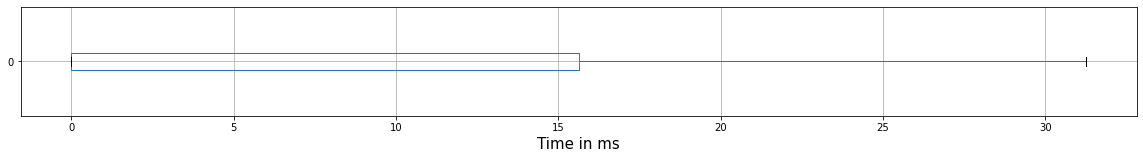
\includegraphics[width=\textwidth,height=\textheight,keepaspectratio]{logos/PurePythonLatencies.png}
     \caption{Time between two frames in a python client}
    \label{fig:PythonFPS}
\end{figure*}
The latencies shown in the following graphs are measured with a video from the
Youtube-8M dataset \parencite{abuelhaija2016}. The video is 4 minutes and 22.94 seconds long and consists of 6,569 frames. Moreover, an average of five replays is used. For consistency, the gaze is fixed in the middle of the frame at the coordinates \((960,512)\). Nevertheless, no loss in latency is measurable when the gaze changes. The overall latency is calculated by sending a time-step from the server to the client. This timestamp is evaluated after the image is shown on the display. This method leads to an overall latency measurement including every step. The image upscaling is at first a linear interpolation. Additionally, the client starts before the server to guarantee an optimal stream initialisation from the beginning.

\begin{table}
\centering
\begin{tabular}{ c | c }
\hline
 Codec & Latency \\ [0.5ex] 
\hline\hline
 WebRTC & ca. 500ms \\ 
 H.265  & ca. 250ms \\  
 H.264  &   >1s     \\  
 VP9    & ca. 1s    \\
 AV1    &   >10s    \\  
\end{tabular}
\caption{Comparison of the latency of the different codecs}
\label{table:comparisoncodecs}
\end{table}


\begin{figure*}[htbp]
    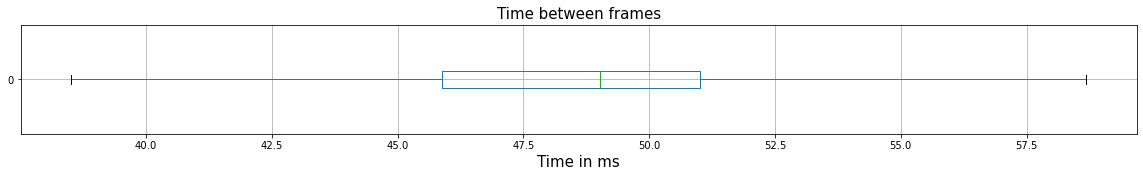
\includegraphics[width=\textwidth,height=\textheight,keepaspectratio]{logos/Unity3DFPS.png}
    \caption{Time between two frames in the Unity3D}
    \label{fig:UnityFPS}
\end{figure*}

\par
After selecting the possible codecs, the different codecs are compared against each other in terms of latency. Stating in \autoref{table:comparisoncodecs}, WebRTC and H.265 achieve the lowest latency. It is to mention that the AV1 codec has currently no hardware encoding and decoding available and therefore is not usable in this setup. Also, the H.264 codec specifies to buffer some frames in any case and cannot be disabled, resulting in this higher latency. As the H.265 is slightly faster with the parameters given in the former section, it was further evaluated. WebRTC could perform better, but due to a time constraint as the implementation differs completely, it was not further considered.
\par

\par
At first, it was proven with \autoref{fig:PythonFPS} that the server and the client deliver constant frames in a specific time limit with a Python client. As seen in \autoref{fig:PythonFPS}, the time between two frames is not more than 30ms, which results in a minimum of 33 FPS. The outliers reach up to 400ms, as the initialisation needs some time and thus the client cannot deliver continuous images during the first few seconds. This scenario is also visible in the image, as it is pixelated in the beginning but then stabilises. The corresponding Unity3D client needs 32–58ms as stated in \autoref{fig:UnityFPS} between each frame and therefore works correctly.

\begin{figure}[htbp]
    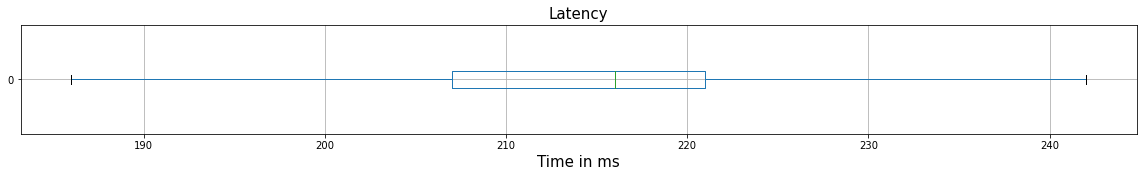
\includegraphics[width=\textwidth,height=\textheight,keepaspectratio]{logos/Unity3dWithoutOutliers.png}
    \caption{Latency of Unity3D}
    \label{fig:UnityLatenyVRWithoutOutliers}
\end{figure}

\begin{figure}[htbp]
    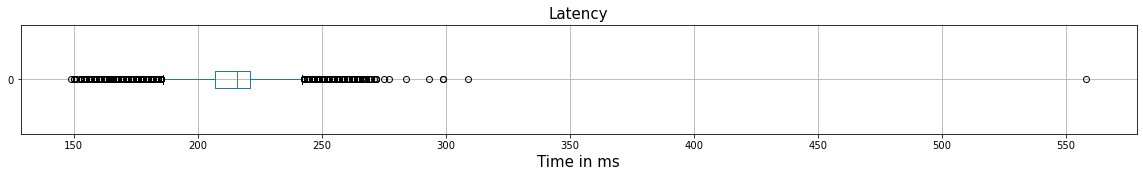
\includegraphics[width=\textwidth,height=\textheight,keepaspectratio]{logos/Unity3dWithOutliers.png}
    \caption{Complete latency of Unity3D with outliers}
    \label{fig:UnityLatenyVRWithOutliers}
\end{figure}

\par 
To measure the latency, different modes were compared. At first, it was determined if there is any impact on the increased hardware demand when the \gls{vr} is enabled or disabled. Furthermore, the differences between the available bandwidths were determined.

\begin{figure}[htbp]
    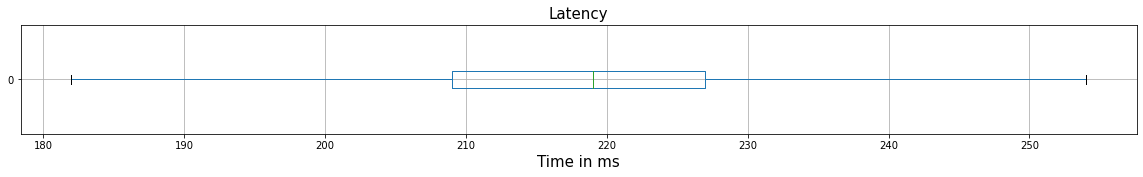
\includegraphics[width=\textwidth,height=\textheight,keepaspectratio]{logos/Unity3dVRWithoutOutliers.png}
    \caption{Latency including enabled\gls{vr}}
    \label{fig:VRLatency}
\end{figure}

\par
When \gls{vr} is disabled and the available bandwidth is not limited, the resulting latency ranges from 172–230ms, whereas the average latency is 219ms as visible in the boxplot of \autoref{fig:UnityLatenyVRWithoutOutliers}. Having a span of 57ms indicates that the transmission is stable, and it also emphasises that there is a continuous frame. Furthermore, there is minimal difference in the latency between when the \gls{vr} is enabled and disabled, which means that the additionally needed hardware power does not impact the streaming as stated in \autoref{fig:VRLatency}.

\begin{figure}[htbp]
    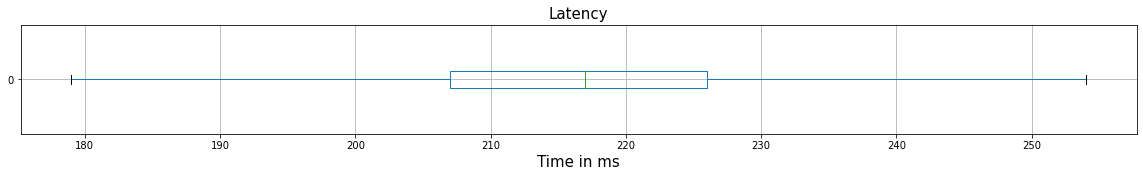
\includegraphics[width=\textwidth,height=\textheight,keepaspectratio]{logos/LowBandwidth.png}
    \caption{Latency with 640 kilobits per second bandwidth}
    \label{fig:lowbandwidthlatency}
\end{figure}

\par
The latency stays the same for a broad span of the available bandwidth. When the bandwidth drops to 640 kilobits per second, the latency does not change as the \autoref{fig:lowbandwidthlatency} indicates. When the rate drops below this line, not every benchmark ran successfully as FFmpeg desynchronised and therefore no stable transmission could be determined.
\par 
The test of the superresolution requires to have a standardised training process. Therefore, each model is trained with 20,000 epochs with the DIVK dataset. The batch size is set to 1 as not more images fit into the VRAM with a crop size of 128. The batch size defines the number of training examples utilized in one training period. In this case, the training example contains two images, a low-resoltion image and the corresponding high-resolution image. As the full training needs at least a day to train, not every model is trained thoroughly. The models differ in the amount of the residual blocks, which repeats 4, 8, 12 or 16 times often. This method allows comparing multiple models for latency. For association, the models are compared against the linear and the bicubic interpolation in terms of latency and quality.

\begin{figure}[htbp]
    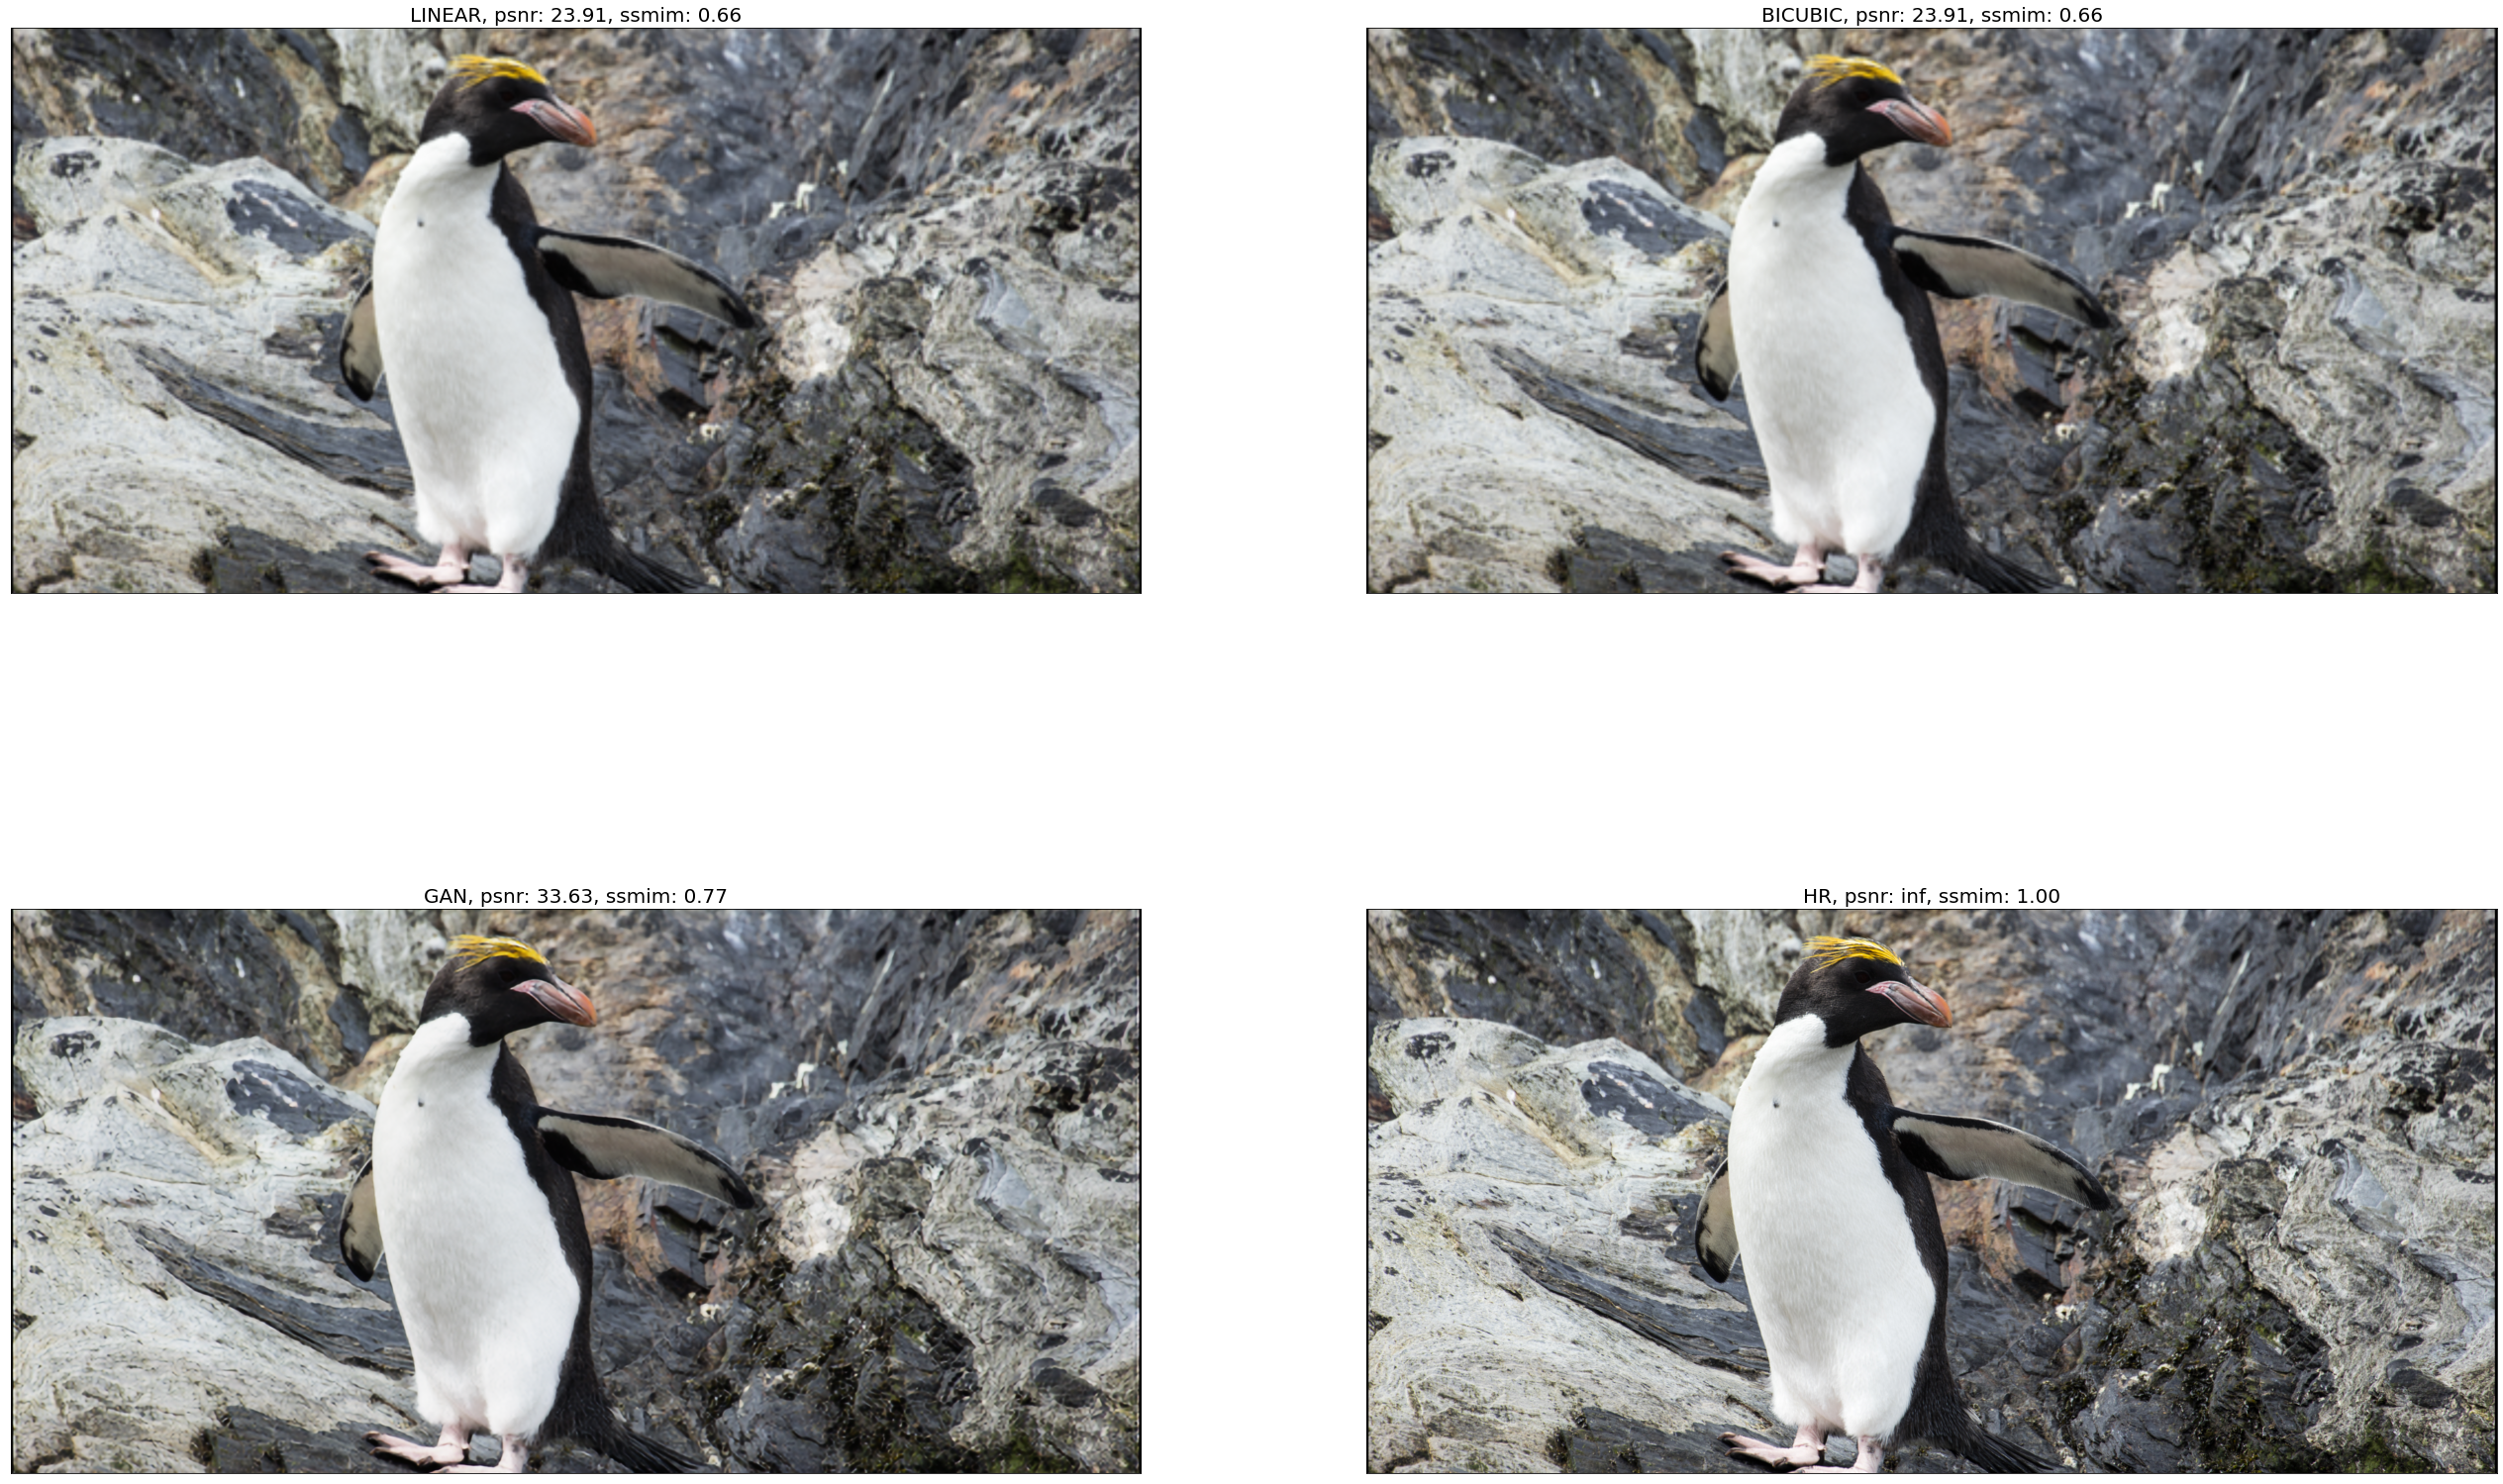
\includegraphics[width=\textwidth,height=\textheight,keepaspectratio]{logos/GANPerformance.png}
    \caption{Performance of a \gls{gan} model in comparison to linear and bicubic interpolation. The image is taken from the DIVK dataset \parencite{Agustsson2017}}
    \label{fig:ganperformance}
\end{figure}

\par
The presented superresolution, which replaces the linear or bicubic upsampling, performs well. It performs the upscaling better than other standard methods. As seen in \autoref{fig:ganperformance}, the peak signal-to-noise ratio (PSNR) value signals the ratio between the maximum possible power of an image and the power of corrupting noise affecting the quality. Moreover, the \gls{ssim} also indicates a better quality, which leads to the result that in terms of superresolution, the neural network beats the standard methods. The speed between the different models differs slightly for a few milliseconds, as stated in \autoref{fig:modellatency}.
\par
Alternatively, the neural network is much slower than the interpolation upsample methods, but it improves the image better. The linear upsampling needs approximately 1ms, which is the fastest method. It delivers acceptable quality in comparison to the neural network, which needs approximately 20ms and creates a better image quality. However, this only relates to the pure network. Furthermore, some other operations add 40ms to the latency, such as a conversation from the float32 type back to the uint8 type, independent of the network.


\begin{figure}[htbp]
    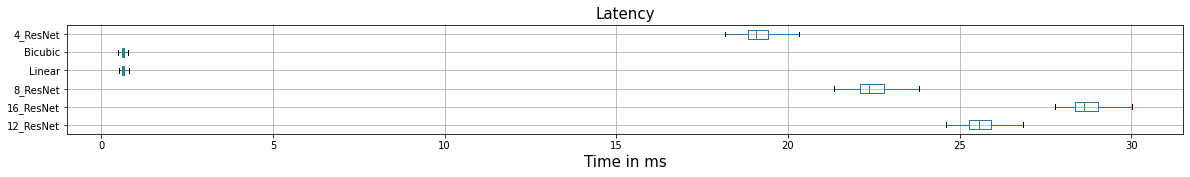
\includegraphics[width=\textwidth,height=\textheight,keepaspectratio]{logos/latencyUpscaling.png}
    \caption{: Latency of the \gls{gan} models in comparison to linear and bicubic interpolation.}
    \label{fig:modellatency}
\end{figure}

\chapter{Conclusion}\label{chapter:conclusion}
In this thesis, a prototype of a streaming solution including foveated rendering and superresolution is developed and evaluated. This chapter describes the results and states the limitations of this work.
\section{Summary}
The proposed solution for optimizing the transmission for limited bandwidth and latency through foveated rendering and superresolution aimed to fulfil many requirements. These requirements are necessary to achieve a streaming solution, which help the user to control the robot appropriately and without having side effects. The first-of-its-kind solution transmits two streams, the foveated region and the peripheral region. Both regions are separated at the server by a received gaze. The separated regions are sent to the client through a specified protocol. The client receives the streams as well as the frame number connected to the gaze and can thus merge the frames correctly. A \gls{hmd} is connected to the client and shows the complete stream in \gls{vr}. The \gls{hmd} also predicts the current gaze and sends it through the client to the server. However, the time constraint of being faster than 125ms was not achieved. In the best case, a single frame is transmitted within 150 milliseconds, and in the worst case, a frame needs approximately 300 milliseconds. Moreover, the superresolution does not achieve its goal to replace the standard interpolation methods appropriately. The problem is the implementation of the superresolution, where the neural network works, but it cannot be implemented as the required additional operations are too time-consuming.
\par
Overall, this attempt to realize a real-time streaming solution with having a latency below 125 milliseconds uncovers many areas about what works and what does not. The presented streaming solution shows that the concept works and provides good results. In contrast, there are problems which have to be solved in future. One of the problems is the large latency, which is great for standard streaming solution but is not usable in the scenario of telepresence.

\section{Limitations}
There are some limitations of this project. One of them is the presented \gls{gan} being large and therefore occupies much \gls{vram}, which results in a small batch size. This also relates to the usability of using the \gls{gan} in a threaded environment. That means when too many images are loaded for superresolution at the same time, the software crashes. This problem also impacts Unity3D reserving also some \gls{vram}. In a single thread scenario, it cannot hold the FPS given as stated in \autoref{fig:UnityFPS}.
\par
As mentioned in the \autoref{chapter:implementation} the optical flow loss was dropped, because of hardware constraints. Facebook used for their training many \glspl{gpu} and still needed round about 48 hours to train the DeepFovea. This indicates that having this large dataset is still challenging for the best computers, even when the training is optimized and distributed.
\par
Finally, the whole project was developed and tested on one machine, leading to a bottleneck at the \gls{gpu}. As two streams are encoded and decoded on this machine as well as the rendering for the \gls{vr} and the \gls{ml} based superresolution a lack of performance is possible. 
\par
Possible solutions are discussed in \autoref{chapter:outlook}. Nevertheless, this project shows that this kind of real-time streaming for telepresence is possible, which is related to controlling a robot.
\chapter{Outlook}\label{chapter:outlook}
There are several possibilities for further improvements. One of them is that the predicted gaze needs some time to the server where the foveated rendering is calculated and then returns to the client. It should be determined whether it is necessary to forecast the gaze for some frames to reach the client faster with the current gaze. This requires that forecasting of the gaze is possible.
\par
Several opportunities exist for improving the latency. The first is to check whether a traditional video codec for compression is required. The encoding and decoding consume most of the latency and is thus the best option for improvements. Facebook uses a spatial matrix for its DeepFovea, which cannot be transmitted by a traditional video platform. Realising a custom transmission protocol to send parts of the matrix would result in more lossy quality but a much faster speed. The matrix can be composed back to an image with the help of a neural network performing superresolution. The proposed neural network must thus change its input type, which would also result in fewer conversations. Additionally, the transmission of the gaze coordinates would be improved as the frame can hold the coordinates by itself, instead of the parallel transmission. Another possibility is to use a neural network codec, which has been proposed recently. These types of codecs also promise to improve the latency by keeping the same quality level, as determined by \cite{Ma2020}.
\par
Moreover, better hardware for floating-point operations, such as the newest GPU generation of Nvidia, promises better machine learning support and faster transcoding \parencite{RTX3000}.



\appendix{}
\newglossaryentry{latex}
{
    name=latex,
    description={Is a mark up language specially suited for scientific documents}
}
\newacronym{ml}{ML}{machine learning}

\newacronym{vr}{VR}{virtual reality}

\newacronym{gan}{GAN}{generative adversarial network}

\newacronym{srgan}{SRGAN}{super resolution generative adversarial network}

\newacronym{wgan}{WGAN}{wassterstein generative adversarial network}

\newacronym{vae}{VAE}{variational autoencoder}

\newacronym{sr}{SR}{superesolution}

\newacronym{em}{EM distance}{Earth-Mover distance}
 
\newacronym{kl}{KL}{Kullback-Leibler divergence}
 
\newacronym{js}{JSD}{Jensen–Shannon divergence}

\newacronym{lpips}{LPIPS}{perceptual image patch similarity}

\newacronym{psnr}{PSNR}{peak signal-to-noise ratio}

\newacronym{ssim}{SSIM}{structural similarity index measure}

\newacronym{hmd}{HMD}{head-mounted display} 

\newacronym{ffr}{FFR}{fixed foveated rendering}

\newacronym{dlss}{DLSS}{deep learning super sampling}

\newacronym{whqd}{WQHD}{Wide Quad HD}

\newacronym{mnist}{MNIST}{Modified  National Institute of Standards and Technology database}

\newacronym{sdk}{SDK}{software development kit}

\newacronym{gpu}{GPU}{graphics processing unit}

\newacronym{cpu}{CPU}{central processing unit}

\newacronym{nvenc}{NVENC}{Nvidia video encoder}

\newacronym{udp}{UDP}{user datagram protocol}

\newacronym{relu}{ReLU}{rectified linear unit}

\newacronym{prelu}{PReLU}{parametric rectified linear unit}

\newacronym{resnet}{ResNet}{residual network}

\newacronym{elu}{ELU}{rectified linear unit}

\newacronym{vram}{VRAM}{video random access memory}

\microtypesetup{protrusion=false}
\listoffigures{}
\listoftables{}
\microtypesetup{protrusion=true}
\printglossary[type=\acronymtype,nonumberlist]
\printbibliography{}
\end{document}
